\documentclass[12pt]{article}

%To do list:
%%1) Fix numbering of reading problems from the reordering, e.g. Lecture 20, q1-->Lecture 18, q1
%%2) Rename webwork sets according to materials not lecture number
%%3) Move images into directories. Here
%%4) Webwork q5 HW6 (in MAT 67 ordering, say <,> for vector notation.
%%5) Problem 6, HW6 has a bug when the eigenvalue is 0.


%%%%%Some commands to make online notes...
\newcommand{\Lecture}{Module}
\newcommand{\moduletitle}[1]{\newpage\thispagestyle{empty}\begin{center}{\LARGE #1}\end{center}}
\newcommand{\modulesection}[1]{\thispagestyle{empty}\section{#1}}
\newcommand{\modulesubsection}[1]{\thispagestyle{empty}\subsection{#1}}
\newcommand{\modulecomment}[1]{}
\newcommand{\moduleobjectives}[1]{#1}
\newcommand{\inputProblems}[1]{}
\newcommand{\moduleinputProblems}[1]{\input{#1}}
\newcommand{\References}[1]{}
\newcommand{\moduletext}[2]{#2}

%use this if you need to show labels, but turn it off afterwards.
%\usepackage{showkeys}
%\usepackage{multimedia}
\usepackage{makeidx}
\usepackage{nopageno} 

\usepackage{comment}
\usepackage{shadow}
\usepackage[english]{babel}
\usepackage{blindtext}
\usepackage{graphicx, color}
\usepackage{tikz}
\DeclareGraphicsRule{*}{mps}{*}{}
\usepackage{linalgjh}
\usepackage{multirow}
\usepackage[colorlinks=true,linkcolor=blue,urlcolor=red,pdfnewwindow=true]{hyperref}
\usepackage[toc]{glossaries}
\usepackage{textcomp}
% Added to work with my enumerates, and I feel that it allows us more flexibility
%  to select how we want to number our items - TCS 1/9/12
\usepackage{enumerate}

\usepackage{linalgdir} % Get the directory and title information

%Change the next line as appropriate for your course.
\newcommand{\webworkurl}{http://webwork.math.ucdavis.edu/webwork2/MAT22A-Waldron-Winter-2012/}
%\newcommand{\webworkurl}{http://webwork.math.ucdavis.edu/webwork2/LinearAlgebra/}
\newcommand{\videourl}{http://math.ucdavis.edu/~linear/videos/}

% This command works by specifying the following (in order):
%  1 - the filename (with extension)
%  2 - the text describing the video
%  3 - The hyperlink reference
% For example we have
% \videoscriptlink{gaussian_elimination_more_background.mp4}{Augmented Matrix Notation~\ref{ge4} and~\ref{ge5}}{script_gaussian_elimination_more}
\newcommand{\videoscriptlink}[3]{
\begin{center}
\href{\videourl #1}{\raisebox{-.4cm}{
\includegraphics[scale=.075]{take1.jpg}}} \hspace{1cm}\scalebox{1.2}{\tt #2}
\hspace{1cm} \hyperlink{#3}{\raisebox{-.3cm}{
\includegraphics[scale=.08]{script.jpg}}}
\end{center}
} % videoscriptlink definition
% I changed all videos I could find to this command - TCS 1/9/12

%%%This links to reading homeworks:
\newcommand{\reading}[2]{\begin{center}
\href{\webworkurl ReadingHomework#1/#2/}{
\raisebox{-3mm}{
\includegraphics[scale=.1]{glasses.jpg}}\hspace{2mm}Reading homework: problem #1.#2}\hspace{8mm}\end{center}}

%%%This links to Mark's videos
\newcommand{\markvideolink}[2]{
\begin{center}
\href{\videourl #1}{\raisebox{-.4cm}{
\includegraphics[scale=.075]{take1.jpg}}} \hspace{1cm}\scalebox{1.2}{\tt #2}
\hspace{1cm} {\raisebox{-.3cm}{\includegraphics[scale=.2]{mark.jpg}}}
\end{center}
}


%%%This links to Kat's videos
\newcommand{\katvideolink}[2]{
\begin{center}
\href{\videourl #1}{\raisebox{-.4cm}{
\includegraphics[scale=.075]{take1.jpg}}} \hspace{1cm}\scalebox{1.2}{\tt #2}
\hspace{1cm} {\raisebox{-.3cm}{\includegraphics[scale=.2]{kat.jpg}}}
\end{center}
}



%A simple URL macro
\newcommand{\URL}[1]{\begin{center}\href{#1}{\tt\scriptsize #1}\end{center}}
\newcommand{\URLS}[2]{\begin{center}\href{#1}{\tt\scriptsize #2}\end{center}}




\def\nn{\nonumber}

\newtheorem{theorem}{Theorem}[section]
\newtheorem{lemma}[theorem]{Lemma}
\newtheorem{proposition}[theorem]{Proposition}
\newtheorem{corollary}[theorem]{Corollary}


\newenvironment{definition}[1][Definition]{\begin{trivlist}
\item[\hskip \labelsep {\bfseries #1}]}{\end{trivlist}}
\newenvironment{example}[1][Example]{\small \sf \begin{trivlist}
\item[\hskip \labelsep {\bfseries #1}]}{\end{trivlist}}
\newenvironment{remark}[1][Remark]{\small \sf \begin{trivlist}
\item[\hskip \labelsep {\bfseries #1}]}{\end{trivlist}}

\DeclareMathOperator{\tr}{tr}
\DeclareMathOperator{\rref}{RREF}

% sideremark
\def\sideremark#1{\ifvmode\leavevmode\fi\vadjust{\vbox to0pt{\vss
\hbox to 0pt{\hskip\hsize\hskip1em
\vbox{\hsize3cm\tiny\raggedright\pretolerance10000
 \noindent #1\hfill}\hss}\vbox to8pt{\vfil}\vss}}}


\newcommand{\edz}[1]{\sideremark{#1}}
\def\idx#1{{\em #1\/}} % ****

\newcommand{\1}{{\rm 1\hspace*{-0.4ex}%
\rule{0.1ex}{1.52ex}\hspace*{0.2ex}}}

\DeclareMathOperator{\cofactor}{cofactor}
\DeclareMathOperator{\spa}{span}
\DeclareMathOperator{\nul}{null}
\newcommand{\phantomnewpage}{}

\makeindex

\makeglossaries


%------------------------------------------------
% TODO LIST
% 0) We moved sections 17,18,19 and 24.
% 1) Reorder WebWork to match section reordering.
% 2) Read through, check for dependency problems.
% 3) Fu's list of corrections
% 4) notes2: Worked example with no solutions
% 
% 
% 


\begin{document}

\pagestyle{plain}

%\newpage

%Testing the video


%\movie[width=8cm,height=10cm]{The Terminator}{videos/vector_spaces_example.mp4}

%\newpage

\tableofcontents

\chapter{\luDecompTitle}
\label{LUdecomp}

Certain matrices are easier to work with than others.  In this section, we will see how to write any square\footnote{The case where $M$ is not square is dealt with at the end of the lecture.} matrix $M$ as the product of two simpler matrices.  We will write $$M=LU\, ,$$ where:
\begin{itemize}
\item $L$ is \emph{lower triangular}\index{Lower triangular matrix}.  This means that all entries above the main diagonal are zero.  In notation,
$L=(l^i_j)$ with $l^i_j=0$ for all $j>i$.
\[L=\begin{pmatrix}
l^1_1 & 0 & 0 & \cdots \\
l^2_1 & l^2_2 & 0 & \cdots \\
l^3_1 & l^3_2 & l^3_3 & \cdots \\
\vdots & \vdots & \vdots & \ddots \\
\end{pmatrix}
\]

\item $U$ is \emph{upper triangular}\index{Upper triangular matrix}.  This means that all entries below the main diagonal are zero.  In notation,
$U=(u^i_j)$ with $u^i_j=0$ for all $j<i$.
\[U=\begin{pmatrix}
u^1_1 & u^1_2 & u^1_3 & \cdots \\
0 & u^2_2 & u^2_3 & \cdots \\
0 & 0 & u^3_3 & \cdots \\
\vdots & \vdots & \vdots & \ddots \\
\end{pmatrix}
\]
\end{itemize}
$M=LU$ is called an \emph{$LU$ decomposition}\index{LU@$LU$ decomposition} of $M$.

This is a useful trick for  computational reasons; it is much easier to compute the inverse of an upper or lower triangular matrix than general matrices.  Since inverses are useful for solving linear systems, this makes solving any linear system associated to the matrix much faster as well.  The determinant---a very important quantity associated with any square matrix---is very easy to compute for triangular matrices.

\begin{example}
Linear systems associated to upper triangular matrices are very easy to solve by back substitution.
\[
\begin{amatrix}{2}
a & b & 1 \\
0 & c & e \\
\end{amatrix} \ \Rightarrow \ y=\frac{e}{c}\, , \quad x=\frac{1}{a}\left(1-\frac{be}{c}\right)
\]

\[
\begin{amatrix}{3}
1 & 0 & 0 & d \\
a & 1 & 0 & e \\
b & c & 1 & f \\
\end{amatrix} \Rightarrow x=d\, , \qquad y=e-ad\, , \qquad z=f-bd-c(e-ad)
\]
For lower triangular matrices, \emph{back} substitution\index{Back substitution} gives a quick solution; for upper triangular matrices, \emph{forward} substitution\index{Forward substitution} gives the solution.
\end{example}





\section{Using $LU$ Decomposition to Solve Linear Systems}

Suppose we have $M=LU$ and want to solve the system
\[
MX=LUX=V.
\]

\begin{itemize}
\item{Step 1:} Set $W=\colvec{u\\v\\w}=UX$.  

\item{Step 2:} Solve the system $LW=V$.  This should be simple by forward substitution since $L$ is lower triangular.  Suppose the solution to $LW=V$ is $W_0$.  

\item{Step 3:} Now solve the system $UX=W_0$.  This should be easy by backward substitution, since $U$ is upper triangular.  The solution to this system is the solution to the original system.
\end{itemize}
We can think of this as using the matrix $L$ to perform row operations on the matrix $U$ in order to solve the system; this idea also appears in the  study of determinants.

%\href{\webworkurl ReadingHomework11/1/}{Reading homework: problem 11.1}
\reading{11}{1}

\begin{example}
Consider the linear system:
\[
      \begin{linsys}{4}
            6x & +&18y & +&3z         &=& 3  \\[1mm]
            2x & +&12y & +&z	    &=& 19 \\[1mm]
            4x & +&15y & +&3z         &=& 0  
      \end{linsys}
\]

An $LU$ decomposition for the associated matrix $M$ is:
\[
\begin{pmatrix}
6 & 18 & 3 \\
2 & 12 & 1 \\
4 & 15 & 3 
\end{pmatrix} =
\begin{pmatrix}
3 & 0 & 0 \\
1 & 6 & 0 \\
2 & 3 & 1 
\end{pmatrix}
\begin{pmatrix}
2 & 6 & 1 \\
0 & 1 & 0 \\
0 & 0 & 1 
\end{pmatrix}.
\]

\begin{itemize}
\item{Step 1:} \hypertarget{LUproc}{Set} $W=\colvec{u\\v\\w}=UX$.  

\item{Step 2:} Solve the system $LW=V$:

\[
\begin{pmatrix}
3 & 0 & 0 \\
1 & 6 & 0 \\
2 & 3 & 1 
\end{pmatrix}
\colvec{u\\v\\w} =
\colvec{3\\19\\0}
\]

By substitution, we get $u=1$, $v=3$, and $w=-11$.  Then 
\[W_0=\colvec{1\\3\\-11}\]

\item{Step 3:} Solve the system $UX=W_0$.  
\[
\begin{pmatrix}
2 & 6 & 1 \\
0 & 1 & 0 \\
0 & 0 & 1 
\end{pmatrix}
\colvec{x\\y\\z} =
\colvec{1\\3\\-11}
\]
Back substitution gives $z=-11, y=3$, and $x=-3$.  

Then $X=\colvec{-3\\3\\-11}$, and we're done.
\end{itemize}
\end{example}

\videoscriptlink{lu_decomposition_using_lu_decomp.mp4}{Using a $LU$ decomposition}{scripts_lu_decomposition_using_lu_example}

%\begin{figure}
\begin{center}
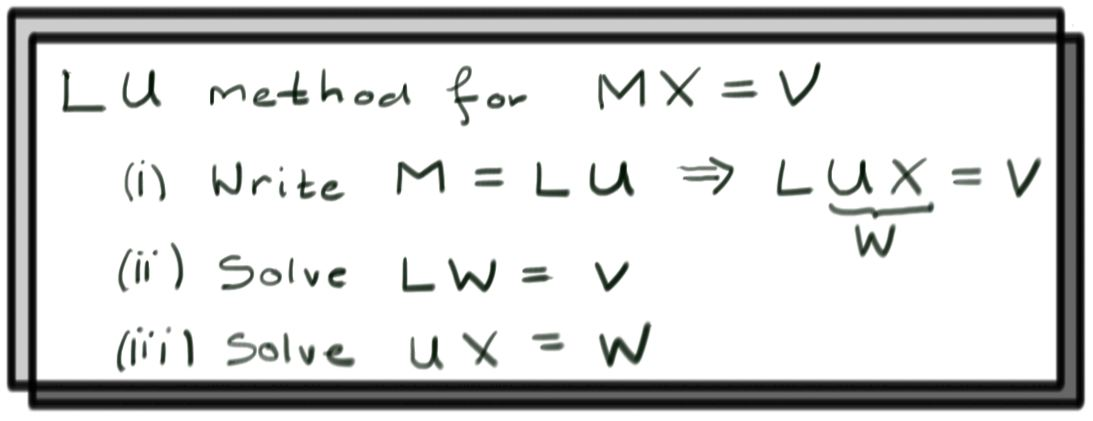
\includegraphics[scale=.3]{\luDecompPath/LU_solution.jpg}
\end{center}
%\end{figure}

\section{Finding an $LU$ Decomposition.}
\label{finding_LU_decomp}
 
For any given matrix, there are actually many different $LU$ decompositions.  However, there is a unique $LU$ decomposition in which the $L$ matrix has ones on the diagonal. In that case $L$ is called a \emph{lower unit triangular matrix}\index{Lower unit triangular matrix}.

To find the $LU$ decomposition, we'll create two sequences of matrices $L_0, L_1, \ldots$ and $U_0, U_1, \ldots$ such that at each step, $L_iU_i=M$.  Each of the $L_i$ will be lower triangular, but only the last $U_i$ will be upper triangular.

Start by setting $L_0=I$ and $U_0=M$, because $L_0U_0=M$. A main concept of this calculation is captured by the following example:

\begin{example}
Consider $$E=\begin{pmatrix}1&0\\\lambda&1\end{pmatrix}\, ,\qquad M=\begin{pmatrix}a&b&c&\cdots\\d&e&f&\cdots\end{pmatrix}\, .$$
Lets compute $EM$
$$
EM=\begin{pmatrix}a&b&c&\cdots\\d+\lambda a&e+\lambda b&f+\lambda c&\cdots\end{pmatrix}\, ,.
$$
Something neat happened here: multiplying $M$ by $E$ performed the row operation $R_2\to R_2+\lambda R-1$ on $M$.
Another interesting fact:
$$
E^{-1}:=\begin{pmatrix}1&0\\-\lambda&1\end{pmatrix}
$$ 
obeys (check this yourself...)
$$
E^{-1} E = 1\, .
$$
Hence $M=E^{-1} E M$ or, writing this out
$$
\begin{pmatrix}a&b&c&\cdots\\d&e&f&\cdots\end{pmatrix}=\begin{pmatrix}1&0\\-\lambda&1\end{pmatrix} \begin{pmatrix}a&b&c&\cdots\\d+\lambda a&e+\lambda b&f+\lambda c&\cdots\end{pmatrix}\, .
$$
Here the matrix on the left is lower triangular, while the matrix on the right has had a row operation performed on it.
\end{example}




\vspace{2mm}
We would like to  use the first row of $U_0$ to zero out the first entry of every row below it.  For our running example, $$U_0=M=\begin{pmatrix}
6 & 18 & 3 \\
2 & 12 & 1 \\
4 & 15 & 3 
\end{pmatrix}\, ,$$ so we would like to perform the row operations $R_2\to R_2 -\frac 13 R_1$ and $R_3\to R_3-\frac 23R_1$.
%so the second row minus $\frac{1}{3}$ of the first row will zero out the first entry in the second row.  Likewise, the third row minus $\frac{2}{3}$ of the first row will zero out the first entry in the third row.
If we perform these row operations on $U_0$ to produce 
$$U_1=\begin{pmatrix}
6 & 18 & 3 \\
0 & 6 & 0 \\
0 & 3 & 1 
\end{pmatrix}\, ,$$
we need to multiply this on the left by a lower triangular matrix $L_1$ so that the product $L_1U_1=M$ still.
The above example shows how to do this:
Set $L_1$ to be the lower triangular matrix whose first column is filled with the minus constants used to zero out the first column of $M$.  Then $$L_1 = \begin{pmatrix}
1 & 0 & 0 \\[1mm]
\frac{1}{3} & 1 & 0 \\[1mm]
\frac{2}{3} & 0 & 1 
\end{pmatrix}\, .$$  
%Set $U_1$ to be the matrix obtained by zeroing out the first column of $M$.  Then $U_1=\begin{pmatrix}
%6 & 18 & 3 \\
%0 & 6 & 0 \\
%0 & 3 & 1 
%\end{pmatrix}$.
By construction $L_1 U_1=M$, but you should compute this yourself as a double check.

Now repeat the process by zeroing the second column of $U_1$ below the diagonal using the second row of $U_1$ using the row operation
$R_3\to R_3-\frac 12 R_2$ to produce
$$U_2=\begin{pmatrix}6&18&3\\0&6&0\\0&0&1\end{pmatrix}\, .$$
The matrix that undoes this row operation is obtained in the same way we found $L_1$ above and is:
$$
\begin{pmatrix}
1&0&0\\
0&1&0\\
0&\frac 12& 0
\end{pmatrix}\, .
$$
Thus our answer for $L_2$ is the product of this matrix with $L_1$, namely
$$
L_2=
\begin{pmatrix}
1 & 0 & 0 \\[1mm]
\frac{1}{3} & 1 & 0 \\[1mm]
\frac{2}{3} & 0 & 1 
\end{pmatrix}\begin{pmatrix}
1&0&0\\
0&1&0\\
0&\frac 12& 0
\end{pmatrix}
=\begin{pmatrix}
1 & 0 & 0 \\[1mm]
\frac{1}{3} & 1 & 0 \\[1mm]
\frac{2}{3} & \frac{1}{2} & 1 
\end{pmatrix}\, .
$$
Notice that it is lower triangular because 

\begin{center}
\textcolor{brown}{THE PRODUCT OF LOWER TRIANGULAR MATRICES IS ALWAYS LOWER TRIANGULAR!}
\end{center}

\noindent
Moreover it is obtained by recording minus the constants used for all our row operations in the appropriate columns (this always works this way).
Moreover, $U_2$ is upper triangular and $M=L_2U_2$, we are done!
Putting this all together we have
$$M=\begin{pmatrix}
6 & 18 & 3 \\
2 & 12 & 1 \\
4 & 15 & 3 
\end{pmatrix}= \begin{pmatrix}
1 & 0 & 0 \\[1mm]
\frac{1}{3} & 1 & 0 \\[1mm]
\frac{2}{3} & \frac{1}{2} & 1 
\end{pmatrix}\begin{pmatrix}
6 & 18 & 3 \\
0 & 6 & 0 \\
0 & 0 & 1 
\end{pmatrix}\, .$$  
%Since $U_2$ is upper-triangular, we're done.  Inserting the new number into $L_1$ to get $L_2$ really is safe: the numbers in the first column don't affect the second column of $U_1$, since the first column of $U_1$ is already zeroed out.

If the matrix you're working with has more than three rows, just continue this process by zeroing out the next column below the diagonal, and repeat until there's nothing left to do.

\videoscriptlink{lu_decomposition_example.mp4}{Another $LU$ decomposition example}{scripts_lu_decomposition_example}

The fractions in the $L$ matrix are admittedly ugly.  For two matrices $LU$, we can multiply one entire column of $L$ by a constant $\lambda$ and divide the corresponding row of $U$ by the same constant without changing the product of the two matrices.  Then:

\begin{eqnarray*}
LU &=& \begin{pmatrix}
1 & 0 & 0 \\[1mm]
\frac{1}{3} & 1 & 0 \\[1mm]
\frac{2}{3} & \frac{1}{2} & 1 
\end{pmatrix}
I
\begin{pmatrix}
6 & 18 & 3 \\
0 & 6 & 0 \\
0 & 0 & 1 
\end{pmatrix} \\
&=&
\begin{pmatrix}
1 & 0 & 0 \\[1mm]
\frac{1}{3} & 1 & 0 \\[1mm]
\frac{2}{3} & \frac{1}{2} & 1 
\end{pmatrix}
\begin{pmatrix}
3 & 0 & 0 \\
0 & 6 & 0 \\
0 & 0 & 1 
\end{pmatrix}
\begin{pmatrix}
\frac{1}{3} & 0 & 0 \\[1mm]
0 & \frac{1}{6} & 0 \\[1mm]
0 & 0 & 1 
\end{pmatrix}
\begin{pmatrix}
6 & 18 & 3 \\
0 & 6 & 0 \\
0 & 0 & 1 
\end{pmatrix} \\
&=&
\begin{pmatrix}
3 & 0 & 0 \\
1 & 6 & 0 \\
2 & 3 & 1 
\end{pmatrix}\begin{pmatrix}
2 & 6 & 1 \\
0 & 1 & 0 \\
0 & 0 & 1 
\end{pmatrix}.
\end{eqnarray*}
The resulting matrix looks nicer, but isn't in standard (lower unit triangular matrix) form.

\reading{11}{2}
%\href{\webworkurl ReadingHomework11/2/}{Reading homework: problem 11.2}

For matrices that are not square, $LU$ decomposition still makes sense.  Given an $m\times n$ matrix $M$, for example we could write $M=LU$ with $L$ a square lower unit triangular matrix, and $U$ a rectangular matrix.  Then $L$ will be an $m\times m$ matrix, and $U$ will be an $m\times n$ matrix (of the same shape as $M$).  From here, the process is exactly the same as for a square matrix.  We create a sequence of matrices $L_i$ and $U_i$ that is eventually the $LU$ decomposition.  Again, we start with $L_0=I$ and $U_0=M$.

\begin{example}
Let's find the $LU$ decomposition of $M=U_0=\begin{pmatrix}
-2 & 1 & 3 \\
-4 & 4 & 1 
\end{pmatrix}$.  Since $M$ is a $2\times 3$ matrix, our decomposition will consist of a $2\times 2$ matrix and a $2\times 3$ matrix.  Then we start with $L_0=I_2=\begin{pmatrix}
1 & 0 \\
0 & 1
\end{pmatrix}$.

The next step is to zero-out the first column of $M$ below the diagonal.  There is only one row to cancel, then, and it can be removed by subtracting $2$ times the first row of $M$ to the second row of $M$.  Then:

\[
L_1=\begin{pmatrix}
1 & 0 \\
2 & 1
\end{pmatrix}, \qquad 
U_1 = \begin{pmatrix}
-2 & 1 & 3 \\
0 & 2 & -5 
\end{pmatrix}
\]
Since $U_1$ is upper triangular, we're done.  With a larger matrix, we would just continue the process.
\end{example}





\section{Block $LDU$ Decomposition}

Let $M$ be a square block matrix with square blocks $X,Y,Z,W$ such that $X^{-1}$ exists.  Then $M$ can be decomposed as a block $LDU$ decomposition, where $D$ is block diagonal, as follows:
\[
M=\begin{pmatrix}
X & Y \\
Z & W
\end{pmatrix}
\]

Then: \[M=\begin{pmatrix}
I &  0 \\
ZX^{-1} & I
\end{pmatrix}\begin{pmatrix}
X & 0 \\
0 & W-ZX^{-1}Y
\end{pmatrix}\begin{pmatrix}
I & X^{-1}Y \\
0 & I
\end{pmatrix}.\]
This can be checked explicitly simply by block-multiplying these three matrices.

\videoscriptlink{lu_decomposition_blocks.mp4}{Block $LDU$ Explanation}{scripts_lu_decomposition_blocks}

\begin{example}
For a $2\times 2$ matrix, we can regard each entry as a block.
\[
\begin{pmatrix}
1 & 2 \\
3 & 4
\end{pmatrix}=
\begin{pmatrix}
1 & 0 \\
3 & 1
\end{pmatrix}
\begin{pmatrix}
1 & 0 \\
0 & -2
\end{pmatrix}
\begin{pmatrix}
1 & 2 \\
0 & 1
\end{pmatrix}
\]
By multiplying the diagonal matrix by the upper triangular matrix, we get the standard $LU$ decomposition of the matrix.
\end{example}


%\section*{References}
%Wikipedia:
%\begin{itemize}
%\item \href{http://en.wikipedia.org/wiki/LU_decomposition}{$LU$ Decomposition}
%\item \href{http://en.wikipedia.org/wiki/Block_LU_decomposition}{Block $LU$ Decomposition}
%\end{itemize}

\section{Review Problems}



\begin{enumerate}

\item Let $D=\begin{pmatrix}
\lambda_1 & \mc0 \\
\mc0 & \lambda_2 \\
\end{pmatrix}$.
\begin{enumerate}
\item Write $D$ in terms of the vectors $e_1$ and $e_2$, and their transposes.
\item Suppose $P=\begin{pmatrix}
a & b \\
c & d \\
\end{pmatrix}$ is invertible.  Show that $D$ is similar to
\[
M=\frac{1}{ad-bc}\begin{pmatrix}
\lambda_1ad-\lambda_2bc & -(\lambda_1-\lambda_2)ab \\[1mm]
(\lambda_1-\lambda_2)cd & -\lambda_1bc + \lambda_2ad
\end{pmatrix}.
\]
\item Suppose the vectors $\rowvec{a,b}$ and $\rowvec{c,d}$ are orthogonal.  What can you say about $M$ in this case? (Hint: think about what \(M^T\) is equal to.)
\end{enumerate}

\phantomnewpage

\item \label{orthogprob} Suppose $S=\{v_1, \ldots, v_n \}$ is an \emph{orthogonal} (not orthonormal) basis for~$\Re^n$.  Then we can write any vector $v$ as $v=\sum_ic^iv_i$ for some constants $c^i$.  Find a formula for the constants $c^i$ in terms of $v$ and the vectors in~$S$.

\Videoscriptlink{orthonormal_bases_hint.mp4}{Hint}{scripts_orthonormal_bases_hint}
\phantomnewpage

\item \label{orthogprojprob} Let $u,v$ be linearly independent vectors in $\Re^3$, and $P=\spa \{ u,v\}$ be the plane spanned by $u$ and $v$.  
\begin{enumerate}
\item Is the vector $v^\bot := v-\frac{u\cdot v}{u\cdot u}u$ in the plane $P$?
\item  What is the (cosine of the) angle between $v^\bot$ and $u$?
\item %Given your solution to the above, 
How can you find a third vector perpendicular to both $u$ and $v^\bot$?
\item  Construct an orthonormal basis for $\Re^3$ from $u$ and $v$.
\item  Test your abstract formul\ae\ starting with 
\[
u=\rowvec{1 , 2 , 0} \text{ and } v=\rowvec{0 , 1 , 1}.
\]
\end{enumerate}

\Videoscriptlink{orthonormal_bases_hint3.mp4}{Hint}{scripts_orthonormal_bases_hint3}

\phantomnewpage



\item Find an orthonormal  basis for $\Re^4$ which includes $(1,1,1,1)$ using the following procedure:\\
\begin{enumerate} 
\item Pick a vector perpendicular to the vector 
$$v_1 =\colvec{1\\1\\1\\1}$$ from the solution set of the matrix equation $$v_1^Tx=0\, .$$ Pick the vector $v_2$ obtained from the standard Gaussian elimination procedure which is the coefficient of $x_2$.
\item Pick a vector perpendicular to both $v_1$ and $v_2$ from the solutions set of the matrix equation $$\colvec{v_1^T\\[1mm]v_2^T}x=0\, .$$ Pick the vector $v_3$ obtained from the standard Gaussian elimination procedure with $x_3$ as the coefficient. 
\item Pick a vector perpendicular to $v_1,v_2,$ and $v_3$ from the solution set of the matrix equation $$\colvec{v_1^T\\[1mm]v_2^T\\[1mm]v_3^T}x=0\, .$$  Pick the vector $v_4$ obtained from the standard Gaussian elimination procedure with $x_3$ as the coefficient. 
\item Normalize the four vectors obtained   above.
\end{enumerate}


\item Use the inner product $$f\cdot g := \int_0^1 f(x)g(x)dx$$  on the vector space $V={\rm span} \{1,x,x^2,x^3\}$ to perform the Gram-Schmidt procedure on the set of vectors $\{1,x,x^2,x^3\}$. 

\item Use the inner product $$f\cdot g := \int_0^{2\pi} f(x)g(x)dx$$  on the vector space $V={\rm span} \{\sin(x),\sin(2x),\sin(3x) \}$ to perform the Gram-Schmidt procedure on the set of vectors $\{\sin(x),\sin(2x),\sin(3x) \}$. \\
Try to build an orthonormal basis for the vector space $$\spa \{ \sin(nx)~| ~n\in \N \}\, .$$
%What do you suspect about the vector space $\spa \{ \sin(nx)~| ~n\in \N \}$?\\
%What do you suspect about the vector space $\spa \{ \sin(ax)~|~ a \in \Re \}$?
\item 
\begin{enumerate}
\item
Show that if $Q$ is an orthogonal $n\times n$ matrix, then $$u\dotprod v = (Qu)\dotprod (Qv)\, ,$$ for any $u,v\in \Re^n$. That is, $Q$ preserves the inner product. 
\item Does $Q$ preserve the outer product? 
\item  If the set of vectors $\{ u_1,\dots,u_n\}$ is orthonormal and $\{ \lambda_1,\cdots,\lambda_n\}$ is a set of numbers, 
then what are the eigenvalues and eigenvectors of the matrix
$M=\sum_{i=1}^n \lambda_i u_i u_i^T$? 
\item How would the eigenvectors and eigenvalues of this matrix change if we replaced  $\{ u_1,\dots,u_n\}$ by $\{ Qu_1,\dots,Q u_n\}$?
\end{enumerate}


\item Carefully write out the Gram-Schmidt procedure for the set of vectors 
$$\left\{ \colvec{1\\1\\1}, \colvec{1\\-1\\1}, \colvec{1\\1\\-1} \right\} \, .$$ Is it possible to rescale the second vector obtained in the procedure to a vector with integer components? 


\item 
\label{basisortho}
\begin{enumerate}
\item Suppose $u$ and $v$ are linearly independent.  Show that $u$ and $v^\perp$ are also linearly independent.  Explain why $\{u, v^\perp\}$ is a basis for $\spa \{u,v\}$.



\Videoscriptlink{gram_schmidt_and_orthogonal_complements_hint.mp4}{Hint}{gram_schmidt_and_orthogonal_complements_hint}

\item Repeat the previous problem, but with three independent vectors $u,v,w$
 where $v^\perp$ and $w^\perp$ are as defined by the Gram-Schmidt procedure. 
\end{enumerate}

\phantomnewpage


\item \label{QRprob} Find the $QR$ factorization of
$$
M=\begin{pmatrix}1&0&\phantom{\!-}2\\-1&2&0\\-1&-2&2
\end{pmatrix}\, .
$$

\phantomnewpage

\item Given any three vectors $u,v,w$, when do $v^\perp$ or $w^\perp$ of the Gram--Schmidt procedure vanish?

\phantomnewpage

\item For $U$ a subspace of $W$, use the subspace theorem to check that $U^\perp$ is a subspace of $W$.

\phantomnewpage


\phantomnewpage

\item %(Extra Credit) 
Let $S_n$ and $A_n$ define the space of $n \times n$ symmetric and anti-symmetric matrices, respectively. These are subspaces of the vector space $M^n_n$ of all $n\times n$ matrices. What is $\dim M^n_n$, $\dim S_n$, and $\dim A_n$? Show that $M^n_n = S_n + A_n$. Define an inner product on square matrices
$$
M\cdot N ={\rm tr} MN\, .
$$
Is $A_n^{\perp}=S_n$? Is $M^n_n = S_n \oplus A_n$?

%\emph{Hint: Note that $\dim S_n = \dim U_n$ where $U_n$ is the vector space of all $n \times n$ upper triangular matrices, and also note that $\dim A_n = \dim \widetilde{U}_n$ where $\widetilde{U}_n$ is the vector space of all strictly $n \times n$ upper triangular matrices (\emph{i.e.} the diagonal entries are all 0).}

\item The vector space $V={\rm span} \{ \sin(t),\sin(2t), \sin(3t) , \sin(3t)\}$ has an inner product: 
$$f\cdot g:=\int _0^{2\pi}f(t)g(t) dt\, .$$ Find the orthogonal compliment to $U={\rm span} \{ \sin(t)+\sin(2t) \}$ in $V$. Express $\sin(t)-\sin(2t)$ as  the sum of vectors from $U$ and $U^\perp$.

\end{enumerate}

\phantomnewpage

\newpage


\chapter{\luDecompTitle}
\label{LUdecomp}

Certain matrices are easier to work with than others.  In this section, we will see how to write any square\footnote{The case where $M$ is not square is dealt with at the end of the lecture.} matrix $M$ as the product of two simpler matrices.  We will write $$M=LU\, ,$$ where:
\begin{itemize}
\item $L$ is \emph{lower triangular}\index{Lower triangular matrix}.  This means that all entries above the main diagonal are zero.  In notation,
$L=(l^i_j)$ with $l^i_j=0$ for all $j>i$.
\[L=\begin{pmatrix}
l^1_1 & 0 & 0 & \cdots \\
l^2_1 & l^2_2 & 0 & \cdots \\
l^3_1 & l^3_2 & l^3_3 & \cdots \\
\vdots & \vdots & \vdots & \ddots \\
\end{pmatrix}
\]

\item $U$ is \emph{upper triangular}\index{Upper triangular matrix}.  This means that all entries below the main diagonal are zero.  In notation,
$U=(u^i_j)$ with $u^i_j=0$ for all $j<i$.
\[U=\begin{pmatrix}
u^1_1 & u^1_2 & u^1_3 & \cdots \\
0 & u^2_2 & u^2_3 & \cdots \\
0 & 0 & u^3_3 & \cdots \\
\vdots & \vdots & \vdots & \ddots \\
\end{pmatrix}
\]
\end{itemize}
$M=LU$ is called an \emph{$LU$ decomposition}\index{LU@$LU$ decomposition} of $M$.

This is a useful trick for  computational reasons; it is much easier to compute the inverse of an upper or lower triangular matrix than general matrices.  Since inverses are useful for solving linear systems, this makes solving any linear system associated to the matrix much faster as well.  The determinant---a very important quantity associated with any square matrix---is very easy to compute for triangular matrices.

\begin{example}
Linear systems associated to upper triangular matrices are very easy to solve by back substitution.
\[
\begin{amatrix}{2}
a & b & 1 \\
0 & c & e \\
\end{amatrix} \ \Rightarrow \ y=\frac{e}{c}\, , \quad x=\frac{1}{a}\left(1-\frac{be}{c}\right)
\]

\[
\begin{amatrix}{3}
1 & 0 & 0 & d \\
a & 1 & 0 & e \\
b & c & 1 & f \\
\end{amatrix} \Rightarrow x=d\, , \qquad y=e-ad\, , \qquad z=f-bd-c(e-ad)
\]
For lower triangular matrices, \emph{back} substitution\index{Back substitution} gives a quick solution; for upper triangular matrices, \emph{forward} substitution\index{Forward substitution} gives the solution.
\end{example}





\section{Using $LU$ Decomposition to Solve Linear Systems}

Suppose we have $M=LU$ and want to solve the system
\[
MX=LUX=V.
\]

\begin{itemize}
\item{Step 1:} Set $W=\colvec{u\\v\\w}=UX$.  

\item{Step 2:} Solve the system $LW=V$.  This should be simple by forward substitution since $L$ is lower triangular.  Suppose the solution to $LW=V$ is $W_0$.  

\item{Step 3:} Now solve the system $UX=W_0$.  This should be easy by backward substitution, since $U$ is upper triangular.  The solution to this system is the solution to the original system.
\end{itemize}
We can think of this as using the matrix $L$ to perform row operations on the matrix $U$ in order to solve the system; this idea also appears in the  study of determinants.

%\href{\webworkurl ReadingHomework11/1/}{Reading homework: problem 11.1}
\reading{11}{1}

\begin{example}
Consider the linear system:
\[
      \begin{linsys}{4}
            6x & +&18y & +&3z         &=& 3  \\[1mm]
            2x & +&12y & +&z	    &=& 19 \\[1mm]
            4x & +&15y & +&3z         &=& 0  
      \end{linsys}
\]

An $LU$ decomposition for the associated matrix $M$ is:
\[
\begin{pmatrix}
6 & 18 & 3 \\
2 & 12 & 1 \\
4 & 15 & 3 
\end{pmatrix} =
\begin{pmatrix}
3 & 0 & 0 \\
1 & 6 & 0 \\
2 & 3 & 1 
\end{pmatrix}
\begin{pmatrix}
2 & 6 & 1 \\
0 & 1 & 0 \\
0 & 0 & 1 
\end{pmatrix}.
\]

\begin{itemize}
\item{Step 1:} \hypertarget{LUproc}{Set} $W=\colvec{u\\v\\w}=UX$.  

\item{Step 2:} Solve the system $LW=V$:

\[
\begin{pmatrix}
3 & 0 & 0 \\
1 & 6 & 0 \\
2 & 3 & 1 
\end{pmatrix}
\colvec{u\\v\\w} =
\colvec{3\\19\\0}
\]

By substitution, we get $u=1$, $v=3$, and $w=-11$.  Then 
\[W_0=\colvec{1\\3\\-11}\]

\item{Step 3:} Solve the system $UX=W_0$.  
\[
\begin{pmatrix}
2 & 6 & 1 \\
0 & 1 & 0 \\
0 & 0 & 1 
\end{pmatrix}
\colvec{x\\y\\z} =
\colvec{1\\3\\-11}
\]
Back substitution gives $z=-11, y=3$, and $x=-3$.  

Then $X=\colvec{-3\\3\\-11}$, and we're done.
\end{itemize}
\end{example}

\videoscriptlink{lu_decomposition_using_lu_decomp.mp4}{Using a $LU$ decomposition}{scripts_lu_decomposition_using_lu_example}

%\begin{figure}
\begin{center}
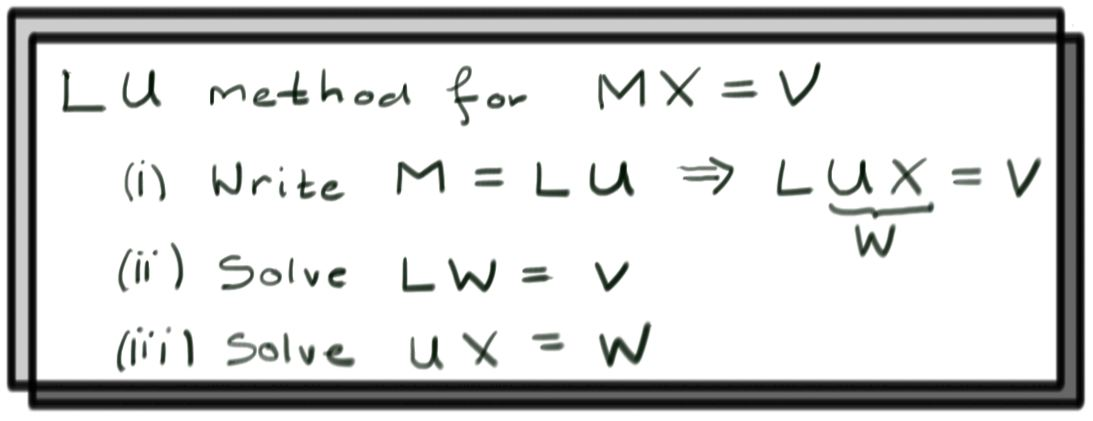
\includegraphics[scale=.3]{\luDecompPath/LU_solution.jpg}
\end{center}
%\end{figure}

\section{Finding an $LU$ Decomposition.}
\label{finding_LU_decomp}
 
For any given matrix, there are actually many different $LU$ decompositions.  However, there is a unique $LU$ decomposition in which the $L$ matrix has ones on the diagonal. In that case $L$ is called a \emph{lower unit triangular matrix}\index{Lower unit triangular matrix}.

To find the $LU$ decomposition, we'll create two sequences of matrices $L_0, L_1, \ldots$ and $U_0, U_1, \ldots$ such that at each step, $L_iU_i=M$.  Each of the $L_i$ will be lower triangular, but only the last $U_i$ will be upper triangular.

Start by setting $L_0=I$ and $U_0=M$, because $L_0U_0=M$. A main concept of this calculation is captured by the following example:

\begin{example}
Consider $$E=\begin{pmatrix}1&0\\\lambda&1\end{pmatrix}\, ,\qquad M=\begin{pmatrix}a&b&c&\cdots\\d&e&f&\cdots\end{pmatrix}\, .$$
Lets compute $EM$
$$
EM=\begin{pmatrix}a&b&c&\cdots\\d+\lambda a&e+\lambda b&f+\lambda c&\cdots\end{pmatrix}\, ,.
$$
Something neat happened here: multiplying $M$ by $E$ performed the row operation $R_2\to R_2+\lambda R-1$ on $M$.
Another interesting fact:
$$
E^{-1}:=\begin{pmatrix}1&0\\-\lambda&1\end{pmatrix}
$$ 
obeys (check this yourself...)
$$
E^{-1} E = 1\, .
$$
Hence $M=E^{-1} E M$ or, writing this out
$$
\begin{pmatrix}a&b&c&\cdots\\d&e&f&\cdots\end{pmatrix}=\begin{pmatrix}1&0\\-\lambda&1\end{pmatrix} \begin{pmatrix}a&b&c&\cdots\\d+\lambda a&e+\lambda b&f+\lambda c&\cdots\end{pmatrix}\, .
$$
Here the matrix on the left is lower triangular, while the matrix on the right has had a row operation performed on it.
\end{example}




\vspace{2mm}
We would like to  use the first row of $U_0$ to zero out the first entry of every row below it.  For our running example, $$U_0=M=\begin{pmatrix}
6 & 18 & 3 \\
2 & 12 & 1 \\
4 & 15 & 3 
\end{pmatrix}\, ,$$ so we would like to perform the row operations $R_2\to R_2 -\frac 13 R_1$ and $R_3\to R_3-\frac 23R_1$.
%so the second row minus $\frac{1}{3}$ of the first row will zero out the first entry in the second row.  Likewise, the third row minus $\frac{2}{3}$ of the first row will zero out the first entry in the third row.
If we perform these row operations on $U_0$ to produce 
$$U_1=\begin{pmatrix}
6 & 18 & 3 \\
0 & 6 & 0 \\
0 & 3 & 1 
\end{pmatrix}\, ,$$
we need to multiply this on the left by a lower triangular matrix $L_1$ so that the product $L_1U_1=M$ still.
The above example shows how to do this:
Set $L_1$ to be the lower triangular matrix whose first column is filled with the minus constants used to zero out the first column of $M$.  Then $$L_1 = \begin{pmatrix}
1 & 0 & 0 \\[1mm]
\frac{1}{3} & 1 & 0 \\[1mm]
\frac{2}{3} & 0 & 1 
\end{pmatrix}\, .$$  
%Set $U_1$ to be the matrix obtained by zeroing out the first column of $M$.  Then $U_1=\begin{pmatrix}
%6 & 18 & 3 \\
%0 & 6 & 0 \\
%0 & 3 & 1 
%\end{pmatrix}$.
By construction $L_1 U_1=M$, but you should compute this yourself as a double check.

Now repeat the process by zeroing the second column of $U_1$ below the diagonal using the second row of $U_1$ using the row operation
$R_3\to R_3-\frac 12 R_2$ to produce
$$U_2=\begin{pmatrix}6&18&3\\0&6&0\\0&0&1\end{pmatrix}\, .$$
The matrix that undoes this row operation is obtained in the same way we found $L_1$ above and is:
$$
\begin{pmatrix}
1&0&0\\
0&1&0\\
0&\frac 12& 0
\end{pmatrix}\, .
$$
Thus our answer for $L_2$ is the product of this matrix with $L_1$, namely
$$
L_2=
\begin{pmatrix}
1 & 0 & 0 \\[1mm]
\frac{1}{3} & 1 & 0 \\[1mm]
\frac{2}{3} & 0 & 1 
\end{pmatrix}\begin{pmatrix}
1&0&0\\
0&1&0\\
0&\frac 12& 0
\end{pmatrix}
=\begin{pmatrix}
1 & 0 & 0 \\[1mm]
\frac{1}{3} & 1 & 0 \\[1mm]
\frac{2}{3} & \frac{1}{2} & 1 
\end{pmatrix}\, .
$$
Notice that it is lower triangular because 

\begin{center}
\textcolor{brown}{THE PRODUCT OF LOWER TRIANGULAR MATRICES IS ALWAYS LOWER TRIANGULAR!}
\end{center}

\noindent
Moreover it is obtained by recording minus the constants used for all our row operations in the appropriate columns (this always works this way).
Moreover, $U_2$ is upper triangular and $M=L_2U_2$, we are done!
Putting this all together we have
$$M=\begin{pmatrix}
6 & 18 & 3 \\
2 & 12 & 1 \\
4 & 15 & 3 
\end{pmatrix}= \begin{pmatrix}
1 & 0 & 0 \\[1mm]
\frac{1}{3} & 1 & 0 \\[1mm]
\frac{2}{3} & \frac{1}{2} & 1 
\end{pmatrix}\begin{pmatrix}
6 & 18 & 3 \\
0 & 6 & 0 \\
0 & 0 & 1 
\end{pmatrix}\, .$$  
%Since $U_2$ is upper-triangular, we're done.  Inserting the new number into $L_1$ to get $L_2$ really is safe: the numbers in the first column don't affect the second column of $U_1$, since the first column of $U_1$ is already zeroed out.

If the matrix you're working with has more than three rows, just continue this process by zeroing out the next column below the diagonal, and repeat until there's nothing left to do.

\videoscriptlink{lu_decomposition_example.mp4}{Another $LU$ decomposition example}{scripts_lu_decomposition_example}

The fractions in the $L$ matrix are admittedly ugly.  For two matrices $LU$, we can multiply one entire column of $L$ by a constant $\lambda$ and divide the corresponding row of $U$ by the same constant without changing the product of the two matrices.  Then:

\begin{eqnarray*}
LU &=& \begin{pmatrix}
1 & 0 & 0 \\[1mm]
\frac{1}{3} & 1 & 0 \\[1mm]
\frac{2}{3} & \frac{1}{2} & 1 
\end{pmatrix}
I
\begin{pmatrix}
6 & 18 & 3 \\
0 & 6 & 0 \\
0 & 0 & 1 
\end{pmatrix} \\
&=&
\begin{pmatrix}
1 & 0 & 0 \\[1mm]
\frac{1}{3} & 1 & 0 \\[1mm]
\frac{2}{3} & \frac{1}{2} & 1 
\end{pmatrix}
\begin{pmatrix}
3 & 0 & 0 \\
0 & 6 & 0 \\
0 & 0 & 1 
\end{pmatrix}
\begin{pmatrix}
\frac{1}{3} & 0 & 0 \\[1mm]
0 & \frac{1}{6} & 0 \\[1mm]
0 & 0 & 1 
\end{pmatrix}
\begin{pmatrix}
6 & 18 & 3 \\
0 & 6 & 0 \\
0 & 0 & 1 
\end{pmatrix} \\
&=&
\begin{pmatrix}
3 & 0 & 0 \\
1 & 6 & 0 \\
2 & 3 & 1 
\end{pmatrix}\begin{pmatrix}
2 & 6 & 1 \\
0 & 1 & 0 \\
0 & 0 & 1 
\end{pmatrix}.
\end{eqnarray*}
The resulting matrix looks nicer, but isn't in standard (lower unit triangular matrix) form.

\reading{11}{2}
%\href{\webworkurl ReadingHomework11/2/}{Reading homework: problem 11.2}

For matrices that are not square, $LU$ decomposition still makes sense.  Given an $m\times n$ matrix $M$, for example we could write $M=LU$ with $L$ a square lower unit triangular matrix, and $U$ a rectangular matrix.  Then $L$ will be an $m\times m$ matrix, and $U$ will be an $m\times n$ matrix (of the same shape as $M$).  From here, the process is exactly the same as for a square matrix.  We create a sequence of matrices $L_i$ and $U_i$ that is eventually the $LU$ decomposition.  Again, we start with $L_0=I$ and $U_0=M$.

\begin{example}
Let's find the $LU$ decomposition of $M=U_0=\begin{pmatrix}
-2 & 1 & 3 \\
-4 & 4 & 1 
\end{pmatrix}$.  Since $M$ is a $2\times 3$ matrix, our decomposition will consist of a $2\times 2$ matrix and a $2\times 3$ matrix.  Then we start with $L_0=I_2=\begin{pmatrix}
1 & 0 \\
0 & 1
\end{pmatrix}$.

The next step is to zero-out the first column of $M$ below the diagonal.  There is only one row to cancel, then, and it can be removed by subtracting $2$ times the first row of $M$ to the second row of $M$.  Then:

\[
L_1=\begin{pmatrix}
1 & 0 \\
2 & 1
\end{pmatrix}, \qquad 
U_1 = \begin{pmatrix}
-2 & 1 & 3 \\
0 & 2 & -5 
\end{pmatrix}
\]
Since $U_1$ is upper triangular, we're done.  With a larger matrix, we would just continue the process.
\end{example}





\section{Block $LDU$ Decomposition}

Let $M$ be a square block matrix with square blocks $X,Y,Z,W$ such that $X^{-1}$ exists.  Then $M$ can be decomposed as a block $LDU$ decomposition, where $D$ is block diagonal, as follows:
\[
M=\begin{pmatrix}
X & Y \\
Z & W
\end{pmatrix}
\]

Then: \[M=\begin{pmatrix}
I &  0 \\
ZX^{-1} & I
\end{pmatrix}\begin{pmatrix}
X & 0 \\
0 & W-ZX^{-1}Y
\end{pmatrix}\begin{pmatrix}
I & X^{-1}Y \\
0 & I
\end{pmatrix}.\]
This can be checked explicitly simply by block-multiplying these three matrices.

\videoscriptlink{lu_decomposition_blocks.mp4}{Block $LDU$ Explanation}{scripts_lu_decomposition_blocks}

\begin{example}
For a $2\times 2$ matrix, we can regard each entry as a block.
\[
\begin{pmatrix}
1 & 2 \\
3 & 4
\end{pmatrix}=
\begin{pmatrix}
1 & 0 \\
3 & 1
\end{pmatrix}
\begin{pmatrix}
1 & 0 \\
0 & -2
\end{pmatrix}
\begin{pmatrix}
1 & 2 \\
0 & 1
\end{pmatrix}
\]
By multiplying the diagonal matrix by the upper triangular matrix, we get the standard $LU$ decomposition of the matrix.
\end{example}


%\section*{References}
%Wikipedia:
%\begin{itemize}
%\item \href{http://en.wikipedia.org/wiki/LU_decomposition}{$LU$ Decomposition}
%\item \href{http://en.wikipedia.org/wiki/Block_LU_decomposition}{Block $LU$ Decomposition}
%\end{itemize}

\section{Review Problems}



\begin{enumerate}

\item Let $D=\begin{pmatrix}
\lambda_1 & \mc0 \\
\mc0 & \lambda_2 \\
\end{pmatrix}$.
\begin{enumerate}
\item Write $D$ in terms of the vectors $e_1$ and $e_2$, and their transposes.
\item Suppose $P=\begin{pmatrix}
a & b \\
c & d \\
\end{pmatrix}$ is invertible.  Show that $D$ is similar to
\[
M=\frac{1}{ad-bc}\begin{pmatrix}
\lambda_1ad-\lambda_2bc & -(\lambda_1-\lambda_2)ab \\[1mm]
(\lambda_1-\lambda_2)cd & -\lambda_1bc + \lambda_2ad
\end{pmatrix}.
\]
\item Suppose the vectors $\rowvec{a,b}$ and $\rowvec{c,d}$ are orthogonal.  What can you say about $M$ in this case? (Hint: think about what \(M^T\) is equal to.)
\end{enumerate}

\phantomnewpage

\item \label{orthogprob} Suppose $S=\{v_1, \ldots, v_n \}$ is an \emph{orthogonal} (not orthonormal) basis for~$\Re^n$.  Then we can write any vector $v$ as $v=\sum_ic^iv_i$ for some constants $c^i$.  Find a formula for the constants $c^i$ in terms of $v$ and the vectors in~$S$.

\Videoscriptlink{orthonormal_bases_hint.mp4}{Hint}{scripts_orthonormal_bases_hint}
\phantomnewpage

\item \label{orthogprojprob} Let $u,v$ be linearly independent vectors in $\Re^3$, and $P=\spa \{ u,v\}$ be the plane spanned by $u$ and $v$.  
\begin{enumerate}
\item Is the vector $v^\bot := v-\frac{u\cdot v}{u\cdot u}u$ in the plane $P$?
\item  What is the (cosine of the) angle between $v^\bot$ and $u$?
\item %Given your solution to the above, 
How can you find a third vector perpendicular to both $u$ and $v^\bot$?
\item  Construct an orthonormal basis for $\Re^3$ from $u$ and $v$.
\item  Test your abstract formul\ae\ starting with 
\[
u=\rowvec{1 , 2 , 0} \text{ and } v=\rowvec{0 , 1 , 1}.
\]
\end{enumerate}

\Videoscriptlink{orthonormal_bases_hint3.mp4}{Hint}{scripts_orthonormal_bases_hint3}

\phantomnewpage



\item Find an orthonormal  basis for $\Re^4$ which includes $(1,1,1,1)$ using the following procedure:\\
\begin{enumerate} 
\item Pick a vector perpendicular to the vector 
$$v_1 =\colvec{1\\1\\1\\1}$$ from the solution set of the matrix equation $$v_1^Tx=0\, .$$ Pick the vector $v_2$ obtained from the standard Gaussian elimination procedure which is the coefficient of $x_2$.
\item Pick a vector perpendicular to both $v_1$ and $v_2$ from the solutions set of the matrix equation $$\colvec{v_1^T\\[1mm]v_2^T}x=0\, .$$ Pick the vector $v_3$ obtained from the standard Gaussian elimination procedure with $x_3$ as the coefficient. 
\item Pick a vector perpendicular to $v_1,v_2,$ and $v_3$ from the solution set of the matrix equation $$\colvec{v_1^T\\[1mm]v_2^T\\[1mm]v_3^T}x=0\, .$$  Pick the vector $v_4$ obtained from the standard Gaussian elimination procedure with $x_3$ as the coefficient. 
\item Normalize the four vectors obtained   above.
\end{enumerate}


\item Use the inner product $$f\cdot g := \int_0^1 f(x)g(x)dx$$  on the vector space $V={\rm span} \{1,x,x^2,x^3\}$ to perform the Gram-Schmidt procedure on the set of vectors $\{1,x,x^2,x^3\}$. 

\item Use the inner product $$f\cdot g := \int_0^{2\pi} f(x)g(x)dx$$  on the vector space $V={\rm span} \{\sin(x),\sin(2x),\sin(3x) \}$ to perform the Gram-Schmidt procedure on the set of vectors $\{\sin(x),\sin(2x),\sin(3x) \}$. \\
Try to build an orthonormal basis for the vector space $$\spa \{ \sin(nx)~| ~n\in \N \}\, .$$
%What do you suspect about the vector space $\spa \{ \sin(nx)~| ~n\in \N \}$?\\
%What do you suspect about the vector space $\spa \{ \sin(ax)~|~ a \in \Re \}$?
\item 
\begin{enumerate}
\item
Show that if $Q$ is an orthogonal $n\times n$ matrix, then $$u\dotprod v = (Qu)\dotprod (Qv)\, ,$$ for any $u,v\in \Re^n$. That is, $Q$ preserves the inner product. 
\item Does $Q$ preserve the outer product? 
\item  If the set of vectors $\{ u_1,\dots,u_n\}$ is orthonormal and $\{ \lambda_1,\cdots,\lambda_n\}$ is a set of numbers, 
then what are the eigenvalues and eigenvectors of the matrix
$M=\sum_{i=1}^n \lambda_i u_i u_i^T$? 
\item How would the eigenvectors and eigenvalues of this matrix change if we replaced  $\{ u_1,\dots,u_n\}$ by $\{ Qu_1,\dots,Q u_n\}$?
\end{enumerate}


\item Carefully write out the Gram-Schmidt procedure for the set of vectors 
$$\left\{ \colvec{1\\1\\1}, \colvec{1\\-1\\1}, \colvec{1\\1\\-1} \right\} \, .$$ Is it possible to rescale the second vector obtained in the procedure to a vector with integer components? 


\item 
\label{basisortho}
\begin{enumerate}
\item Suppose $u$ and $v$ are linearly independent.  Show that $u$ and $v^\perp$ are also linearly independent.  Explain why $\{u, v^\perp\}$ is a basis for $\spa \{u,v\}$.



\Videoscriptlink{gram_schmidt_and_orthogonal_complements_hint.mp4}{Hint}{gram_schmidt_and_orthogonal_complements_hint}

\item Repeat the previous problem, but with three independent vectors $u,v,w$
 where $v^\perp$ and $w^\perp$ are as defined by the Gram-Schmidt procedure. 
\end{enumerate}

\phantomnewpage


\item \label{QRprob} Find the $QR$ factorization of
$$
M=\begin{pmatrix}1&0&\phantom{\!-}2\\-1&2&0\\-1&-2&2
\end{pmatrix}\, .
$$

\phantomnewpage

\item Given any three vectors $u,v,w$, when do $v^\perp$ or $w^\perp$ of the Gram--Schmidt procedure vanish?

\phantomnewpage

\item For $U$ a subspace of $W$, use the subspace theorem to check that $U^\perp$ is a subspace of $W$.

\phantomnewpage


\phantomnewpage

\item %(Extra Credit) 
Let $S_n$ and $A_n$ define the space of $n \times n$ symmetric and anti-symmetric matrices, respectively. These are subspaces of the vector space $M^n_n$ of all $n\times n$ matrices. What is $\dim M^n_n$, $\dim S_n$, and $\dim A_n$? Show that $M^n_n = S_n + A_n$. Define an inner product on square matrices
$$
M\cdot N ={\rm tr} MN\, .
$$
Is $A_n^{\perp}=S_n$? Is $M^n_n = S_n \oplus A_n$?

%\emph{Hint: Note that $\dim S_n = \dim U_n$ where $U_n$ is the vector space of all $n \times n$ upper triangular matrices, and also note that $\dim A_n = \dim \widetilde{U}_n$ where $\widetilde{U}_n$ is the vector space of all strictly $n \times n$ upper triangular matrices (\emph{i.e.} the diagonal entries are all 0).}

\item The vector space $V={\rm span} \{ \sin(t),\sin(2t), \sin(3t) , \sin(3t)\}$ has an inner product: 
$$f\cdot g:=\int _0^{2\pi}f(t)g(t) dt\, .$$ Find the orthogonal compliment to $U={\rm span} \{ \sin(t)+\sin(2t) \}$ in $V$. Express $\sin(t)-\sin(2t)$ as  the sum of vectors from $U$ and $U^\perp$.

\end{enumerate}

\phantomnewpage

\newpage


\chapter{\luDecompTitle}
\label{LUdecomp}

Certain matrices are easier to work with than others.  In this section, we will see how to write any square\footnote{The case where $M$ is not square is dealt with at the end of the lecture.} matrix $M$ as the product of two simpler matrices.  We will write $$M=LU\, ,$$ where:
\begin{itemize}
\item $L$ is \emph{lower triangular}\index{Lower triangular matrix}.  This means that all entries above the main diagonal are zero.  In notation,
$L=(l^i_j)$ with $l^i_j=0$ for all $j>i$.
\[L=\begin{pmatrix}
l^1_1 & 0 & 0 & \cdots \\
l^2_1 & l^2_2 & 0 & \cdots \\
l^3_1 & l^3_2 & l^3_3 & \cdots \\
\vdots & \vdots & \vdots & \ddots \\
\end{pmatrix}
\]

\item $U$ is \emph{upper triangular}\index{Upper triangular matrix}.  This means that all entries below the main diagonal are zero.  In notation,
$U=(u^i_j)$ with $u^i_j=0$ for all $j<i$.
\[U=\begin{pmatrix}
u^1_1 & u^1_2 & u^1_3 & \cdots \\
0 & u^2_2 & u^2_3 & \cdots \\
0 & 0 & u^3_3 & \cdots \\
\vdots & \vdots & \vdots & \ddots \\
\end{pmatrix}
\]
\end{itemize}
$M=LU$ is called an \emph{$LU$ decomposition}\index{LU@$LU$ decomposition} of $M$.

This is a useful trick for  computational reasons; it is much easier to compute the inverse of an upper or lower triangular matrix than general matrices.  Since inverses are useful for solving linear systems, this makes solving any linear system associated to the matrix much faster as well.  The determinant---a very important quantity associated with any square matrix---is very easy to compute for triangular matrices.

\begin{example}
Linear systems associated to upper triangular matrices are very easy to solve by back substitution.
\[
\begin{amatrix}{2}
a & b & 1 \\
0 & c & e \\
\end{amatrix} \ \Rightarrow \ y=\frac{e}{c}\, , \quad x=\frac{1}{a}\left(1-\frac{be}{c}\right)
\]

\[
\begin{amatrix}{3}
1 & 0 & 0 & d \\
a & 1 & 0 & e \\
b & c & 1 & f \\
\end{amatrix} \Rightarrow x=d\, , \qquad y=e-ad\, , \qquad z=f-bd-c(e-ad)
\]
For lower triangular matrices, \emph{back} substitution\index{Back substitution} gives a quick solution; for upper triangular matrices, \emph{forward} substitution\index{Forward substitution} gives the solution.
\end{example}





\section{Using $LU$ Decomposition to Solve Linear Systems}

Suppose we have $M=LU$ and want to solve the system
\[
MX=LUX=V.
\]

\begin{itemize}
\item{Step 1:} Set $W=\colvec{u\\v\\w}=UX$.  

\item{Step 2:} Solve the system $LW=V$.  This should be simple by forward substitution since $L$ is lower triangular.  Suppose the solution to $LW=V$ is $W_0$.  

\item{Step 3:} Now solve the system $UX=W_0$.  This should be easy by backward substitution, since $U$ is upper triangular.  The solution to this system is the solution to the original system.
\end{itemize}
We can think of this as using the matrix $L$ to perform row operations on the matrix $U$ in order to solve the system; this idea also appears in the  study of determinants.

%\href{\webworkurl ReadingHomework11/1/}{Reading homework: problem 11.1}
\reading{11}{1}

\begin{example}
Consider the linear system:
\[
      \begin{linsys}{4}
            6x & +&18y & +&3z         &=& 3  \\[1mm]
            2x & +&12y & +&z	    &=& 19 \\[1mm]
            4x & +&15y & +&3z         &=& 0  
      \end{linsys}
\]

An $LU$ decomposition for the associated matrix $M$ is:
\[
\begin{pmatrix}
6 & 18 & 3 \\
2 & 12 & 1 \\
4 & 15 & 3 
\end{pmatrix} =
\begin{pmatrix}
3 & 0 & 0 \\
1 & 6 & 0 \\
2 & 3 & 1 
\end{pmatrix}
\begin{pmatrix}
2 & 6 & 1 \\
0 & 1 & 0 \\
0 & 0 & 1 
\end{pmatrix}.
\]

\begin{itemize}
\item{Step 1:} \hypertarget{LUproc}{Set} $W=\colvec{u\\v\\w}=UX$.  

\item{Step 2:} Solve the system $LW=V$:

\[
\begin{pmatrix}
3 & 0 & 0 \\
1 & 6 & 0 \\
2 & 3 & 1 
\end{pmatrix}
\colvec{u\\v\\w} =
\colvec{3\\19\\0}
\]

By substitution, we get $u=1$, $v=3$, and $w=-11$.  Then 
\[W_0=\colvec{1\\3\\-11}\]

\item{Step 3:} Solve the system $UX=W_0$.  
\[
\begin{pmatrix}
2 & 6 & 1 \\
0 & 1 & 0 \\
0 & 0 & 1 
\end{pmatrix}
\colvec{x\\y\\z} =
\colvec{1\\3\\-11}
\]
Back substitution gives $z=-11, y=3$, and $x=-3$.  

Then $X=\colvec{-3\\3\\-11}$, and we're done.
\end{itemize}
\end{example}

\videoscriptlink{lu_decomposition_using_lu_decomp.mp4}{Using a $LU$ decomposition}{scripts_lu_decomposition_using_lu_example}

%\begin{figure}
\begin{center}
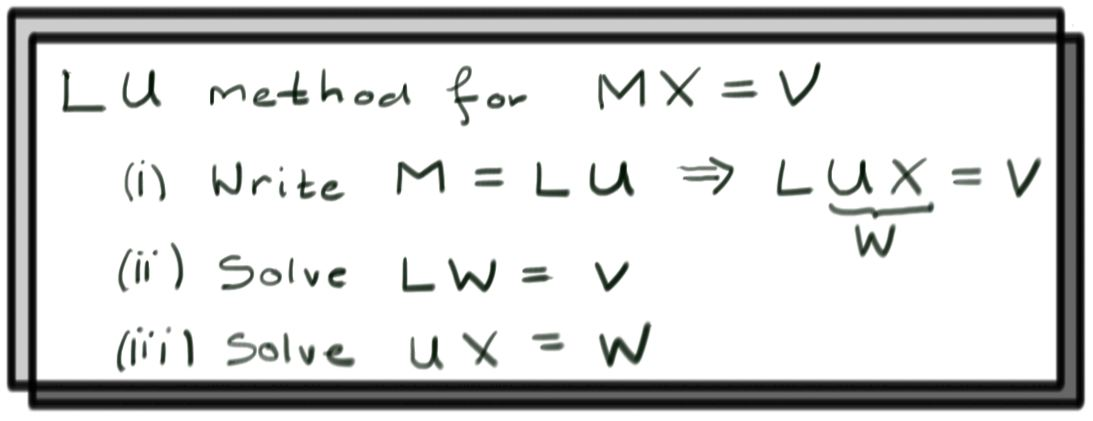
\includegraphics[scale=.3]{\luDecompPath/LU_solution.jpg}
\end{center}
%\end{figure}

\section{Finding an $LU$ Decomposition.}
\label{finding_LU_decomp}
 
For any given matrix, there are actually many different $LU$ decompositions.  However, there is a unique $LU$ decomposition in which the $L$ matrix has ones on the diagonal. In that case $L$ is called a \emph{lower unit triangular matrix}\index{Lower unit triangular matrix}.

To find the $LU$ decomposition, we'll create two sequences of matrices $L_0, L_1, \ldots$ and $U_0, U_1, \ldots$ such that at each step, $L_iU_i=M$.  Each of the $L_i$ will be lower triangular, but only the last $U_i$ will be upper triangular.

Start by setting $L_0=I$ and $U_0=M$, because $L_0U_0=M$. A main concept of this calculation is captured by the following example:

\begin{example}
Consider $$E=\begin{pmatrix}1&0\\\lambda&1\end{pmatrix}\, ,\qquad M=\begin{pmatrix}a&b&c&\cdots\\d&e&f&\cdots\end{pmatrix}\, .$$
Lets compute $EM$
$$
EM=\begin{pmatrix}a&b&c&\cdots\\d+\lambda a&e+\lambda b&f+\lambda c&\cdots\end{pmatrix}\, ,.
$$
Something neat happened here: multiplying $M$ by $E$ performed the row operation $R_2\to R_2+\lambda R-1$ on $M$.
Another interesting fact:
$$
E^{-1}:=\begin{pmatrix}1&0\\-\lambda&1\end{pmatrix}
$$ 
obeys (check this yourself...)
$$
E^{-1} E = 1\, .
$$
Hence $M=E^{-1} E M$ or, writing this out
$$
\begin{pmatrix}a&b&c&\cdots\\d&e&f&\cdots\end{pmatrix}=\begin{pmatrix}1&0\\-\lambda&1\end{pmatrix} \begin{pmatrix}a&b&c&\cdots\\d+\lambda a&e+\lambda b&f+\lambda c&\cdots\end{pmatrix}\, .
$$
Here the matrix on the left is lower triangular, while the matrix on the right has had a row operation performed on it.
\end{example}




\vspace{2mm}
We would like to  use the first row of $U_0$ to zero out the first entry of every row below it.  For our running example, $$U_0=M=\begin{pmatrix}
6 & 18 & 3 \\
2 & 12 & 1 \\
4 & 15 & 3 
\end{pmatrix}\, ,$$ so we would like to perform the row operations $R_2\to R_2 -\frac 13 R_1$ and $R_3\to R_3-\frac 23R_1$.
%so the second row minus $\frac{1}{3}$ of the first row will zero out the first entry in the second row.  Likewise, the third row minus $\frac{2}{3}$ of the first row will zero out the first entry in the third row.
If we perform these row operations on $U_0$ to produce 
$$U_1=\begin{pmatrix}
6 & 18 & 3 \\
0 & 6 & 0 \\
0 & 3 & 1 
\end{pmatrix}\, ,$$
we need to multiply this on the left by a lower triangular matrix $L_1$ so that the product $L_1U_1=M$ still.
The above example shows how to do this:
Set $L_1$ to be the lower triangular matrix whose first column is filled with the minus constants used to zero out the first column of $M$.  Then $$L_1 = \begin{pmatrix}
1 & 0 & 0 \\[1mm]
\frac{1}{3} & 1 & 0 \\[1mm]
\frac{2}{3} & 0 & 1 
\end{pmatrix}\, .$$  
%Set $U_1$ to be the matrix obtained by zeroing out the first column of $M$.  Then $U_1=\begin{pmatrix}
%6 & 18 & 3 \\
%0 & 6 & 0 \\
%0 & 3 & 1 
%\end{pmatrix}$.
By construction $L_1 U_1=M$, but you should compute this yourself as a double check.

Now repeat the process by zeroing the second column of $U_1$ below the diagonal using the second row of $U_1$ using the row operation
$R_3\to R_3-\frac 12 R_2$ to produce
$$U_2=\begin{pmatrix}6&18&3\\0&6&0\\0&0&1\end{pmatrix}\, .$$
The matrix that undoes this row operation is obtained in the same way we found $L_1$ above and is:
$$
\begin{pmatrix}
1&0&0\\
0&1&0\\
0&\frac 12& 0
\end{pmatrix}\, .
$$
Thus our answer for $L_2$ is the product of this matrix with $L_1$, namely
$$
L_2=
\begin{pmatrix}
1 & 0 & 0 \\[1mm]
\frac{1}{3} & 1 & 0 \\[1mm]
\frac{2}{3} & 0 & 1 
\end{pmatrix}\begin{pmatrix}
1&0&0\\
0&1&0\\
0&\frac 12& 0
\end{pmatrix}
=\begin{pmatrix}
1 & 0 & 0 \\[1mm]
\frac{1}{3} & 1 & 0 \\[1mm]
\frac{2}{3} & \frac{1}{2} & 1 
\end{pmatrix}\, .
$$
Notice that it is lower triangular because 

\begin{center}
\textcolor{brown}{THE PRODUCT OF LOWER TRIANGULAR MATRICES IS ALWAYS LOWER TRIANGULAR!}
\end{center}

\noindent
Moreover it is obtained by recording minus the constants used for all our row operations in the appropriate columns (this always works this way).
Moreover, $U_2$ is upper triangular and $M=L_2U_2$, we are done!
Putting this all together we have
$$M=\begin{pmatrix}
6 & 18 & 3 \\
2 & 12 & 1 \\
4 & 15 & 3 
\end{pmatrix}= \begin{pmatrix}
1 & 0 & 0 \\[1mm]
\frac{1}{3} & 1 & 0 \\[1mm]
\frac{2}{3} & \frac{1}{2} & 1 
\end{pmatrix}\begin{pmatrix}
6 & 18 & 3 \\
0 & 6 & 0 \\
0 & 0 & 1 
\end{pmatrix}\, .$$  
%Since $U_2$ is upper-triangular, we're done.  Inserting the new number into $L_1$ to get $L_2$ really is safe: the numbers in the first column don't affect the second column of $U_1$, since the first column of $U_1$ is already zeroed out.

If the matrix you're working with has more than three rows, just continue this process by zeroing out the next column below the diagonal, and repeat until there's nothing left to do.

\videoscriptlink{lu_decomposition_example.mp4}{Another $LU$ decomposition example}{scripts_lu_decomposition_example}

The fractions in the $L$ matrix are admittedly ugly.  For two matrices $LU$, we can multiply one entire column of $L$ by a constant $\lambda$ and divide the corresponding row of $U$ by the same constant without changing the product of the two matrices.  Then:

\begin{eqnarray*}
LU &=& \begin{pmatrix}
1 & 0 & 0 \\[1mm]
\frac{1}{3} & 1 & 0 \\[1mm]
\frac{2}{3} & \frac{1}{2} & 1 
\end{pmatrix}
I
\begin{pmatrix}
6 & 18 & 3 \\
0 & 6 & 0 \\
0 & 0 & 1 
\end{pmatrix} \\
&=&
\begin{pmatrix}
1 & 0 & 0 \\[1mm]
\frac{1}{3} & 1 & 0 \\[1mm]
\frac{2}{3} & \frac{1}{2} & 1 
\end{pmatrix}
\begin{pmatrix}
3 & 0 & 0 \\
0 & 6 & 0 \\
0 & 0 & 1 
\end{pmatrix}
\begin{pmatrix}
\frac{1}{3} & 0 & 0 \\[1mm]
0 & \frac{1}{6} & 0 \\[1mm]
0 & 0 & 1 
\end{pmatrix}
\begin{pmatrix}
6 & 18 & 3 \\
0 & 6 & 0 \\
0 & 0 & 1 
\end{pmatrix} \\
&=&
\begin{pmatrix}
3 & 0 & 0 \\
1 & 6 & 0 \\
2 & 3 & 1 
\end{pmatrix}\begin{pmatrix}
2 & 6 & 1 \\
0 & 1 & 0 \\
0 & 0 & 1 
\end{pmatrix}.
\end{eqnarray*}
The resulting matrix looks nicer, but isn't in standard (lower unit triangular matrix) form.

\reading{11}{2}
%\href{\webworkurl ReadingHomework11/2/}{Reading homework: problem 11.2}

For matrices that are not square, $LU$ decomposition still makes sense.  Given an $m\times n$ matrix $M$, for example we could write $M=LU$ with $L$ a square lower unit triangular matrix, and $U$ a rectangular matrix.  Then $L$ will be an $m\times m$ matrix, and $U$ will be an $m\times n$ matrix (of the same shape as $M$).  From here, the process is exactly the same as for a square matrix.  We create a sequence of matrices $L_i$ and $U_i$ that is eventually the $LU$ decomposition.  Again, we start with $L_0=I$ and $U_0=M$.

\begin{example}
Let's find the $LU$ decomposition of $M=U_0=\begin{pmatrix}
-2 & 1 & 3 \\
-4 & 4 & 1 
\end{pmatrix}$.  Since $M$ is a $2\times 3$ matrix, our decomposition will consist of a $2\times 2$ matrix and a $2\times 3$ matrix.  Then we start with $L_0=I_2=\begin{pmatrix}
1 & 0 \\
0 & 1
\end{pmatrix}$.

The next step is to zero-out the first column of $M$ below the diagonal.  There is only one row to cancel, then, and it can be removed by subtracting $2$ times the first row of $M$ to the second row of $M$.  Then:

\[
L_1=\begin{pmatrix}
1 & 0 \\
2 & 1
\end{pmatrix}, \qquad 
U_1 = \begin{pmatrix}
-2 & 1 & 3 \\
0 & 2 & -5 
\end{pmatrix}
\]
Since $U_1$ is upper triangular, we're done.  With a larger matrix, we would just continue the process.
\end{example}





\section{Block $LDU$ Decomposition}

Let $M$ be a square block matrix with square blocks $X,Y,Z,W$ such that $X^{-1}$ exists.  Then $M$ can be decomposed as a block $LDU$ decomposition, where $D$ is block diagonal, as follows:
\[
M=\begin{pmatrix}
X & Y \\
Z & W
\end{pmatrix}
\]

Then: \[M=\begin{pmatrix}
I &  0 \\
ZX^{-1} & I
\end{pmatrix}\begin{pmatrix}
X & 0 \\
0 & W-ZX^{-1}Y
\end{pmatrix}\begin{pmatrix}
I & X^{-1}Y \\
0 & I
\end{pmatrix}.\]
This can be checked explicitly simply by block-multiplying these three matrices.

\videoscriptlink{lu_decomposition_blocks.mp4}{Block $LDU$ Explanation}{scripts_lu_decomposition_blocks}

\begin{example}
For a $2\times 2$ matrix, we can regard each entry as a block.
\[
\begin{pmatrix}
1 & 2 \\
3 & 4
\end{pmatrix}=
\begin{pmatrix}
1 & 0 \\
3 & 1
\end{pmatrix}
\begin{pmatrix}
1 & 0 \\
0 & -2
\end{pmatrix}
\begin{pmatrix}
1 & 2 \\
0 & 1
\end{pmatrix}
\]
By multiplying the diagonal matrix by the upper triangular matrix, we get the standard $LU$ decomposition of the matrix.
\end{example}


%\section*{References}
%Wikipedia:
%\begin{itemize}
%\item \href{http://en.wikipedia.org/wiki/LU_decomposition}{$LU$ Decomposition}
%\item \href{http://en.wikipedia.org/wiki/Block_LU_decomposition}{Block $LU$ Decomposition}
%\end{itemize}

\section{Review Problems}



\begin{enumerate}

\item Let $D=\begin{pmatrix}
\lambda_1 & \mc0 \\
\mc0 & \lambda_2 \\
\end{pmatrix}$.
\begin{enumerate}
\item Write $D$ in terms of the vectors $e_1$ and $e_2$, and their transposes.
\item Suppose $P=\begin{pmatrix}
a & b \\
c & d \\
\end{pmatrix}$ is invertible.  Show that $D$ is similar to
\[
M=\frac{1}{ad-bc}\begin{pmatrix}
\lambda_1ad-\lambda_2bc & -(\lambda_1-\lambda_2)ab \\[1mm]
(\lambda_1-\lambda_2)cd & -\lambda_1bc + \lambda_2ad
\end{pmatrix}.
\]
\item Suppose the vectors $\rowvec{a,b}$ and $\rowvec{c,d}$ are orthogonal.  What can you say about $M$ in this case? (Hint: think about what \(M^T\) is equal to.)
\end{enumerate}

\phantomnewpage

\item \label{orthogprob} Suppose $S=\{v_1, \ldots, v_n \}$ is an \emph{orthogonal} (not orthonormal) basis for~$\Re^n$.  Then we can write any vector $v$ as $v=\sum_ic^iv_i$ for some constants $c^i$.  Find a formula for the constants $c^i$ in terms of $v$ and the vectors in~$S$.

\Videoscriptlink{orthonormal_bases_hint.mp4}{Hint}{scripts_orthonormal_bases_hint}
\phantomnewpage

\item \label{orthogprojprob} Let $u,v$ be linearly independent vectors in $\Re^3$, and $P=\spa \{ u,v\}$ be the plane spanned by $u$ and $v$.  
\begin{enumerate}
\item Is the vector $v^\bot := v-\frac{u\cdot v}{u\cdot u}u$ in the plane $P$?
\item  What is the (cosine of the) angle between $v^\bot$ and $u$?
\item %Given your solution to the above, 
How can you find a third vector perpendicular to both $u$ and $v^\bot$?
\item  Construct an orthonormal basis for $\Re^3$ from $u$ and $v$.
\item  Test your abstract formul\ae\ starting with 
\[
u=\rowvec{1 , 2 , 0} \text{ and } v=\rowvec{0 , 1 , 1}.
\]
\end{enumerate}

\Videoscriptlink{orthonormal_bases_hint3.mp4}{Hint}{scripts_orthonormal_bases_hint3}

\phantomnewpage



\item Find an orthonormal  basis for $\Re^4$ which includes $(1,1,1,1)$ using the following procedure:\\
\begin{enumerate} 
\item Pick a vector perpendicular to the vector 
$$v_1 =\colvec{1\\1\\1\\1}$$ from the solution set of the matrix equation $$v_1^Tx=0\, .$$ Pick the vector $v_2$ obtained from the standard Gaussian elimination procedure which is the coefficient of $x_2$.
\item Pick a vector perpendicular to both $v_1$ and $v_2$ from the solutions set of the matrix equation $$\colvec{v_1^T\\[1mm]v_2^T}x=0\, .$$ Pick the vector $v_3$ obtained from the standard Gaussian elimination procedure with $x_3$ as the coefficient. 
\item Pick a vector perpendicular to $v_1,v_2,$ and $v_3$ from the solution set of the matrix equation $$\colvec{v_1^T\\[1mm]v_2^T\\[1mm]v_3^T}x=0\, .$$  Pick the vector $v_4$ obtained from the standard Gaussian elimination procedure with $x_3$ as the coefficient. 
\item Normalize the four vectors obtained   above.
\end{enumerate}


\item Use the inner product $$f\cdot g := \int_0^1 f(x)g(x)dx$$  on the vector space $V={\rm span} \{1,x,x^2,x^3\}$ to perform the Gram-Schmidt procedure on the set of vectors $\{1,x,x^2,x^3\}$. 

\item Use the inner product $$f\cdot g := \int_0^{2\pi} f(x)g(x)dx$$  on the vector space $V={\rm span} \{\sin(x),\sin(2x),\sin(3x) \}$ to perform the Gram-Schmidt procedure on the set of vectors $\{\sin(x),\sin(2x),\sin(3x) \}$. \\
Try to build an orthonormal basis for the vector space $$\spa \{ \sin(nx)~| ~n\in \N \}\, .$$
%What do you suspect about the vector space $\spa \{ \sin(nx)~| ~n\in \N \}$?\\
%What do you suspect about the vector space $\spa \{ \sin(ax)~|~ a \in \Re \}$?
\item 
\begin{enumerate}
\item
Show that if $Q$ is an orthogonal $n\times n$ matrix, then $$u\dotprod v = (Qu)\dotprod (Qv)\, ,$$ for any $u,v\in \Re^n$. That is, $Q$ preserves the inner product. 
\item Does $Q$ preserve the outer product? 
\item  If the set of vectors $\{ u_1,\dots,u_n\}$ is orthonormal and $\{ \lambda_1,\cdots,\lambda_n\}$ is a set of numbers, 
then what are the eigenvalues and eigenvectors of the matrix
$M=\sum_{i=1}^n \lambda_i u_i u_i^T$? 
\item How would the eigenvectors and eigenvalues of this matrix change if we replaced  $\{ u_1,\dots,u_n\}$ by $\{ Qu_1,\dots,Q u_n\}$?
\end{enumerate}


\item Carefully write out the Gram-Schmidt procedure for the set of vectors 
$$\left\{ \colvec{1\\1\\1}, \colvec{1\\-1\\1}, \colvec{1\\1\\-1} \right\} \, .$$ Is it possible to rescale the second vector obtained in the procedure to a vector with integer components? 


\item 
\label{basisortho}
\begin{enumerate}
\item Suppose $u$ and $v$ are linearly independent.  Show that $u$ and $v^\perp$ are also linearly independent.  Explain why $\{u, v^\perp\}$ is a basis for $\spa \{u,v\}$.



\Videoscriptlink{gram_schmidt_and_orthogonal_complements_hint.mp4}{Hint}{gram_schmidt_and_orthogonal_complements_hint}

\item Repeat the previous problem, but with three independent vectors $u,v,w$
 where $v^\perp$ and $w^\perp$ are as defined by the Gram-Schmidt procedure. 
\end{enumerate}

\phantomnewpage


\item \label{QRprob} Find the $QR$ factorization of
$$
M=\begin{pmatrix}1&0&\phantom{\!-}2\\-1&2&0\\-1&-2&2
\end{pmatrix}\, .
$$

\phantomnewpage

\item Given any three vectors $u,v,w$, when do $v^\perp$ or $w^\perp$ of the Gram--Schmidt procedure vanish?

\phantomnewpage

\item For $U$ a subspace of $W$, use the subspace theorem to check that $U^\perp$ is a subspace of $W$.

\phantomnewpage


\phantomnewpage

\item %(Extra Credit) 
Let $S_n$ and $A_n$ define the space of $n \times n$ symmetric and anti-symmetric matrices, respectively. These are subspaces of the vector space $M^n_n$ of all $n\times n$ matrices. What is $\dim M^n_n$, $\dim S_n$, and $\dim A_n$? Show that $M^n_n = S_n + A_n$. Define an inner product on square matrices
$$
M\cdot N ={\rm tr} MN\, .
$$
Is $A_n^{\perp}=S_n$? Is $M^n_n = S_n \oplus A_n$?

%\emph{Hint: Note that $\dim S_n = \dim U_n$ where $U_n$ is the vector space of all $n \times n$ upper triangular matrices, and also note that $\dim A_n = \dim \widetilde{U}_n$ where $\widetilde{U}_n$ is the vector space of all strictly $n \times n$ upper triangular matrices (\emph{i.e.} the diagonal entries are all 0).}

\item The vector space $V={\rm span} \{ \sin(t),\sin(2t), \sin(3t) , \sin(3t)\}$ has an inner product: 
$$f\cdot g:=\int _0^{2\pi}f(t)g(t) dt\, .$$ Find the orthogonal compliment to $U={\rm span} \{ \sin(t)+\sin(2t) \}$ in $V$. Express $\sin(t)-\sin(2t)$ as  the sum of vectors from $U$ and $U^\perp$.

\end{enumerate}

\phantomnewpage

\newpage


\chapter{\luDecompTitle}
\label{LUdecomp}

Certain matrices are easier to work with than others.  In this section, we will see how to write any square\footnote{The case where $M$ is not square is dealt with at the end of the lecture.} matrix $M$ as the product of two simpler matrices.  We will write $$M=LU\, ,$$ where:
\begin{itemize}
\item $L$ is \emph{lower triangular}\index{Lower triangular matrix}.  This means that all entries above the main diagonal are zero.  In notation,
$L=(l^i_j)$ with $l^i_j=0$ for all $j>i$.
\[L=\begin{pmatrix}
l^1_1 & 0 & 0 & \cdots \\
l^2_1 & l^2_2 & 0 & \cdots \\
l^3_1 & l^3_2 & l^3_3 & \cdots \\
\vdots & \vdots & \vdots & \ddots \\
\end{pmatrix}
\]

\item $U$ is \emph{upper triangular}\index{Upper triangular matrix}.  This means that all entries below the main diagonal are zero.  In notation,
$U=(u^i_j)$ with $u^i_j=0$ for all $j<i$.
\[U=\begin{pmatrix}
u^1_1 & u^1_2 & u^1_3 & \cdots \\
0 & u^2_2 & u^2_3 & \cdots \\
0 & 0 & u^3_3 & \cdots \\
\vdots & \vdots & \vdots & \ddots \\
\end{pmatrix}
\]
\end{itemize}
$M=LU$ is called an \emph{$LU$ decomposition}\index{LU@$LU$ decomposition} of $M$.

This is a useful trick for  computational reasons; it is much easier to compute the inverse of an upper or lower triangular matrix than general matrices.  Since inverses are useful for solving linear systems, this makes solving any linear system associated to the matrix much faster as well.  The determinant---a very important quantity associated with any square matrix---is very easy to compute for triangular matrices.

\begin{example}
Linear systems associated to upper triangular matrices are very easy to solve by back substitution.
\[
\begin{amatrix}{2}
a & b & 1 \\
0 & c & e \\
\end{amatrix} \ \Rightarrow \ y=\frac{e}{c}\, , \quad x=\frac{1}{a}\left(1-\frac{be}{c}\right)
\]

\[
\begin{amatrix}{3}
1 & 0 & 0 & d \\
a & 1 & 0 & e \\
b & c & 1 & f \\
\end{amatrix} \Rightarrow x=d\, , \qquad y=e-ad\, , \qquad z=f-bd-c(e-ad)
\]
For lower triangular matrices, \emph{back} substitution\index{Back substitution} gives a quick solution; for upper triangular matrices, \emph{forward} substitution\index{Forward substitution} gives the solution.
\end{example}





\section{Using $LU$ Decomposition to Solve Linear Systems}

Suppose we have $M=LU$ and want to solve the system
\[
MX=LUX=V.
\]

\begin{itemize}
\item{Step 1:} Set $W=\colvec{u\\v\\w}=UX$.  

\item{Step 2:} Solve the system $LW=V$.  This should be simple by forward substitution since $L$ is lower triangular.  Suppose the solution to $LW=V$ is $W_0$.  

\item{Step 3:} Now solve the system $UX=W_0$.  This should be easy by backward substitution, since $U$ is upper triangular.  The solution to this system is the solution to the original system.
\end{itemize}
We can think of this as using the matrix $L$ to perform row operations on the matrix $U$ in order to solve the system; this idea also appears in the  study of determinants.

%\href{\webworkurl ReadingHomework11/1/}{Reading homework: problem 11.1}
\reading{11}{1}

\begin{example}
Consider the linear system:
\[
      \begin{linsys}{4}
            6x & +&18y & +&3z         &=& 3  \\[1mm]
            2x & +&12y & +&z	    &=& 19 \\[1mm]
            4x & +&15y & +&3z         &=& 0  
      \end{linsys}
\]

An $LU$ decomposition for the associated matrix $M$ is:
\[
\begin{pmatrix}
6 & 18 & 3 \\
2 & 12 & 1 \\
4 & 15 & 3 
\end{pmatrix} =
\begin{pmatrix}
3 & 0 & 0 \\
1 & 6 & 0 \\
2 & 3 & 1 
\end{pmatrix}
\begin{pmatrix}
2 & 6 & 1 \\
0 & 1 & 0 \\
0 & 0 & 1 
\end{pmatrix}.
\]

\begin{itemize}
\item{Step 1:} \hypertarget{LUproc}{Set} $W=\colvec{u\\v\\w}=UX$.  

\item{Step 2:} Solve the system $LW=V$:

\[
\begin{pmatrix}
3 & 0 & 0 \\
1 & 6 & 0 \\
2 & 3 & 1 
\end{pmatrix}
\colvec{u\\v\\w} =
\colvec{3\\19\\0}
\]

By substitution, we get $u=1$, $v=3$, and $w=-11$.  Then 
\[W_0=\colvec{1\\3\\-11}\]

\item{Step 3:} Solve the system $UX=W_0$.  
\[
\begin{pmatrix}
2 & 6 & 1 \\
0 & 1 & 0 \\
0 & 0 & 1 
\end{pmatrix}
\colvec{x\\y\\z} =
\colvec{1\\3\\-11}
\]
Back substitution gives $z=-11, y=3$, and $x=-3$.  

Then $X=\colvec{-3\\3\\-11}$, and we're done.
\end{itemize}
\end{example}

\videoscriptlink{lu_decomposition_using_lu_decomp.mp4}{Using a $LU$ decomposition}{scripts_lu_decomposition_using_lu_example}

%\begin{figure}
\begin{center}
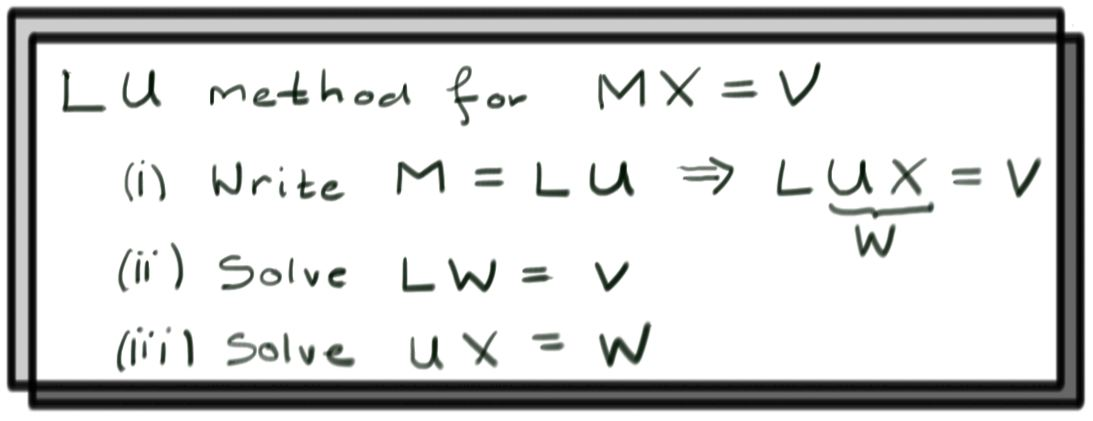
\includegraphics[scale=.3]{\luDecompPath/LU_solution.jpg}
\end{center}
%\end{figure}

\section{Finding an $LU$ Decomposition.}
\label{finding_LU_decomp}
 
For any given matrix, there are actually many different $LU$ decompositions.  However, there is a unique $LU$ decomposition in which the $L$ matrix has ones on the diagonal. In that case $L$ is called a \emph{lower unit triangular matrix}\index{Lower unit triangular matrix}.

To find the $LU$ decomposition, we'll create two sequences of matrices $L_0, L_1, \ldots$ and $U_0, U_1, \ldots$ such that at each step, $L_iU_i=M$.  Each of the $L_i$ will be lower triangular, but only the last $U_i$ will be upper triangular.

Start by setting $L_0=I$ and $U_0=M$, because $L_0U_0=M$. A main concept of this calculation is captured by the following example:

\begin{example}
Consider $$E=\begin{pmatrix}1&0\\\lambda&1\end{pmatrix}\, ,\qquad M=\begin{pmatrix}a&b&c&\cdots\\d&e&f&\cdots\end{pmatrix}\, .$$
Lets compute $EM$
$$
EM=\begin{pmatrix}a&b&c&\cdots\\d+\lambda a&e+\lambda b&f+\lambda c&\cdots\end{pmatrix}\, ,.
$$
Something neat happened here: multiplying $M$ by $E$ performed the row operation $R_2\to R_2+\lambda R-1$ on $M$.
Another interesting fact:
$$
E^{-1}:=\begin{pmatrix}1&0\\-\lambda&1\end{pmatrix}
$$ 
obeys (check this yourself...)
$$
E^{-1} E = 1\, .
$$
Hence $M=E^{-1} E M$ or, writing this out
$$
\begin{pmatrix}a&b&c&\cdots\\d&e&f&\cdots\end{pmatrix}=\begin{pmatrix}1&0\\-\lambda&1\end{pmatrix} \begin{pmatrix}a&b&c&\cdots\\d+\lambda a&e+\lambda b&f+\lambda c&\cdots\end{pmatrix}\, .
$$
Here the matrix on the left is lower triangular, while the matrix on the right has had a row operation performed on it.
\end{example}




\vspace{2mm}
We would like to  use the first row of $U_0$ to zero out the first entry of every row below it.  For our running example, $$U_0=M=\begin{pmatrix}
6 & 18 & 3 \\
2 & 12 & 1 \\
4 & 15 & 3 
\end{pmatrix}\, ,$$ so we would like to perform the row operations $R_2\to R_2 -\frac 13 R_1$ and $R_3\to R_3-\frac 23R_1$.
%so the second row minus $\frac{1}{3}$ of the first row will zero out the first entry in the second row.  Likewise, the third row minus $\frac{2}{3}$ of the first row will zero out the first entry in the third row.
If we perform these row operations on $U_0$ to produce 
$$U_1=\begin{pmatrix}
6 & 18 & 3 \\
0 & 6 & 0 \\
0 & 3 & 1 
\end{pmatrix}\, ,$$
we need to multiply this on the left by a lower triangular matrix $L_1$ so that the product $L_1U_1=M$ still.
The above example shows how to do this:
Set $L_1$ to be the lower triangular matrix whose first column is filled with the minus constants used to zero out the first column of $M$.  Then $$L_1 = \begin{pmatrix}
1 & 0 & 0 \\[1mm]
\frac{1}{3} & 1 & 0 \\[1mm]
\frac{2}{3} & 0 & 1 
\end{pmatrix}\, .$$  
%Set $U_1$ to be the matrix obtained by zeroing out the first column of $M$.  Then $U_1=\begin{pmatrix}
%6 & 18 & 3 \\
%0 & 6 & 0 \\
%0 & 3 & 1 
%\end{pmatrix}$.
By construction $L_1 U_1=M$, but you should compute this yourself as a double check.

Now repeat the process by zeroing the second column of $U_1$ below the diagonal using the second row of $U_1$ using the row operation
$R_3\to R_3-\frac 12 R_2$ to produce
$$U_2=\begin{pmatrix}6&18&3\\0&6&0\\0&0&1\end{pmatrix}\, .$$
The matrix that undoes this row operation is obtained in the same way we found $L_1$ above and is:
$$
\begin{pmatrix}
1&0&0\\
0&1&0\\
0&\frac 12& 0
\end{pmatrix}\, .
$$
Thus our answer for $L_2$ is the product of this matrix with $L_1$, namely
$$
L_2=
\begin{pmatrix}
1 & 0 & 0 \\[1mm]
\frac{1}{3} & 1 & 0 \\[1mm]
\frac{2}{3} & 0 & 1 
\end{pmatrix}\begin{pmatrix}
1&0&0\\
0&1&0\\
0&\frac 12& 0
\end{pmatrix}
=\begin{pmatrix}
1 & 0 & 0 \\[1mm]
\frac{1}{3} & 1 & 0 \\[1mm]
\frac{2}{3} & \frac{1}{2} & 1 
\end{pmatrix}\, .
$$
Notice that it is lower triangular because 

\begin{center}
\textcolor{brown}{THE PRODUCT OF LOWER TRIANGULAR MATRICES IS ALWAYS LOWER TRIANGULAR!}
\end{center}

\noindent
Moreover it is obtained by recording minus the constants used for all our row operations in the appropriate columns (this always works this way).
Moreover, $U_2$ is upper triangular and $M=L_2U_2$, we are done!
Putting this all together we have
$$M=\begin{pmatrix}
6 & 18 & 3 \\
2 & 12 & 1 \\
4 & 15 & 3 
\end{pmatrix}= \begin{pmatrix}
1 & 0 & 0 \\[1mm]
\frac{1}{3} & 1 & 0 \\[1mm]
\frac{2}{3} & \frac{1}{2} & 1 
\end{pmatrix}\begin{pmatrix}
6 & 18 & 3 \\
0 & 6 & 0 \\
0 & 0 & 1 
\end{pmatrix}\, .$$  
%Since $U_2$ is upper-triangular, we're done.  Inserting the new number into $L_1$ to get $L_2$ really is safe: the numbers in the first column don't affect the second column of $U_1$, since the first column of $U_1$ is already zeroed out.

If the matrix you're working with has more than three rows, just continue this process by zeroing out the next column below the diagonal, and repeat until there's nothing left to do.

\videoscriptlink{lu_decomposition_example.mp4}{Another $LU$ decomposition example}{scripts_lu_decomposition_example}

The fractions in the $L$ matrix are admittedly ugly.  For two matrices $LU$, we can multiply one entire column of $L$ by a constant $\lambda$ and divide the corresponding row of $U$ by the same constant without changing the product of the two matrices.  Then:

\begin{eqnarray*}
LU &=& \begin{pmatrix}
1 & 0 & 0 \\[1mm]
\frac{1}{3} & 1 & 0 \\[1mm]
\frac{2}{3} & \frac{1}{2} & 1 
\end{pmatrix}
I
\begin{pmatrix}
6 & 18 & 3 \\
0 & 6 & 0 \\
0 & 0 & 1 
\end{pmatrix} \\
&=&
\begin{pmatrix}
1 & 0 & 0 \\[1mm]
\frac{1}{3} & 1 & 0 \\[1mm]
\frac{2}{3} & \frac{1}{2} & 1 
\end{pmatrix}
\begin{pmatrix}
3 & 0 & 0 \\
0 & 6 & 0 \\
0 & 0 & 1 
\end{pmatrix}
\begin{pmatrix}
\frac{1}{3} & 0 & 0 \\[1mm]
0 & \frac{1}{6} & 0 \\[1mm]
0 & 0 & 1 
\end{pmatrix}
\begin{pmatrix}
6 & 18 & 3 \\
0 & 6 & 0 \\
0 & 0 & 1 
\end{pmatrix} \\
&=&
\begin{pmatrix}
3 & 0 & 0 \\
1 & 6 & 0 \\
2 & 3 & 1 
\end{pmatrix}\begin{pmatrix}
2 & 6 & 1 \\
0 & 1 & 0 \\
0 & 0 & 1 
\end{pmatrix}.
\end{eqnarray*}
The resulting matrix looks nicer, but isn't in standard (lower unit triangular matrix) form.

\reading{11}{2}
%\href{\webworkurl ReadingHomework11/2/}{Reading homework: problem 11.2}

For matrices that are not square, $LU$ decomposition still makes sense.  Given an $m\times n$ matrix $M$, for example we could write $M=LU$ with $L$ a square lower unit triangular matrix, and $U$ a rectangular matrix.  Then $L$ will be an $m\times m$ matrix, and $U$ will be an $m\times n$ matrix (of the same shape as $M$).  From here, the process is exactly the same as for a square matrix.  We create a sequence of matrices $L_i$ and $U_i$ that is eventually the $LU$ decomposition.  Again, we start with $L_0=I$ and $U_0=M$.

\begin{example}
Let's find the $LU$ decomposition of $M=U_0=\begin{pmatrix}
-2 & 1 & 3 \\
-4 & 4 & 1 
\end{pmatrix}$.  Since $M$ is a $2\times 3$ matrix, our decomposition will consist of a $2\times 2$ matrix and a $2\times 3$ matrix.  Then we start with $L_0=I_2=\begin{pmatrix}
1 & 0 \\
0 & 1
\end{pmatrix}$.

The next step is to zero-out the first column of $M$ below the diagonal.  There is only one row to cancel, then, and it can be removed by subtracting $2$ times the first row of $M$ to the second row of $M$.  Then:

\[
L_1=\begin{pmatrix}
1 & 0 \\
2 & 1
\end{pmatrix}, \qquad 
U_1 = \begin{pmatrix}
-2 & 1 & 3 \\
0 & 2 & -5 
\end{pmatrix}
\]
Since $U_1$ is upper triangular, we're done.  With a larger matrix, we would just continue the process.
\end{example}





\section{Block $LDU$ Decomposition}

Let $M$ be a square block matrix with square blocks $X,Y,Z,W$ such that $X^{-1}$ exists.  Then $M$ can be decomposed as a block $LDU$ decomposition, where $D$ is block diagonal, as follows:
\[
M=\begin{pmatrix}
X & Y \\
Z & W
\end{pmatrix}
\]

Then: \[M=\begin{pmatrix}
I &  0 \\
ZX^{-1} & I
\end{pmatrix}\begin{pmatrix}
X & 0 \\
0 & W-ZX^{-1}Y
\end{pmatrix}\begin{pmatrix}
I & X^{-1}Y \\
0 & I
\end{pmatrix}.\]
This can be checked explicitly simply by block-multiplying these three matrices.

\videoscriptlink{lu_decomposition_blocks.mp4}{Block $LDU$ Explanation}{scripts_lu_decomposition_blocks}

\begin{example}
For a $2\times 2$ matrix, we can regard each entry as a block.
\[
\begin{pmatrix}
1 & 2 \\
3 & 4
\end{pmatrix}=
\begin{pmatrix}
1 & 0 \\
3 & 1
\end{pmatrix}
\begin{pmatrix}
1 & 0 \\
0 & -2
\end{pmatrix}
\begin{pmatrix}
1 & 2 \\
0 & 1
\end{pmatrix}
\]
By multiplying the diagonal matrix by the upper triangular matrix, we get the standard $LU$ decomposition of the matrix.
\end{example}


%\section*{References}
%Wikipedia:
%\begin{itemize}
%\item \href{http://en.wikipedia.org/wiki/LU_decomposition}{$LU$ Decomposition}
%\item \href{http://en.wikipedia.org/wiki/Block_LU_decomposition}{Block $LU$ Decomposition}
%\end{itemize}

\section{Review Problems}



\begin{enumerate}

\item Let $D=\begin{pmatrix}
\lambda_1 & \mc0 \\
\mc0 & \lambda_2 \\
\end{pmatrix}$.
\begin{enumerate}
\item Write $D$ in terms of the vectors $e_1$ and $e_2$, and their transposes.
\item Suppose $P=\begin{pmatrix}
a & b \\
c & d \\
\end{pmatrix}$ is invertible.  Show that $D$ is similar to
\[
M=\frac{1}{ad-bc}\begin{pmatrix}
\lambda_1ad-\lambda_2bc & -(\lambda_1-\lambda_2)ab \\[1mm]
(\lambda_1-\lambda_2)cd & -\lambda_1bc + \lambda_2ad
\end{pmatrix}.
\]
\item Suppose the vectors $\rowvec{a,b}$ and $\rowvec{c,d}$ are orthogonal.  What can you say about $M$ in this case? (Hint: think about what \(M^T\) is equal to.)
\end{enumerate}

\phantomnewpage

\item \label{orthogprob} Suppose $S=\{v_1, \ldots, v_n \}$ is an \emph{orthogonal} (not orthonormal) basis for~$\Re^n$.  Then we can write any vector $v$ as $v=\sum_ic^iv_i$ for some constants $c^i$.  Find a formula for the constants $c^i$ in terms of $v$ and the vectors in~$S$.

\Videoscriptlink{orthonormal_bases_hint.mp4}{Hint}{scripts_orthonormal_bases_hint}
\phantomnewpage

\item \label{orthogprojprob} Let $u,v$ be linearly independent vectors in $\Re^3$, and $P=\spa \{ u,v\}$ be the plane spanned by $u$ and $v$.  
\begin{enumerate}
\item Is the vector $v^\bot := v-\frac{u\cdot v}{u\cdot u}u$ in the plane $P$?
\item  What is the (cosine of the) angle between $v^\bot$ and $u$?
\item %Given your solution to the above, 
How can you find a third vector perpendicular to both $u$ and $v^\bot$?
\item  Construct an orthonormal basis for $\Re^3$ from $u$ and $v$.
\item  Test your abstract formul\ae\ starting with 
\[
u=\rowvec{1 , 2 , 0} \text{ and } v=\rowvec{0 , 1 , 1}.
\]
\end{enumerate}

\Videoscriptlink{orthonormal_bases_hint3.mp4}{Hint}{scripts_orthonormal_bases_hint3}

\phantomnewpage



\item Find an orthonormal  basis for $\Re^4$ which includes $(1,1,1,1)$ using the following procedure:\\
\begin{enumerate} 
\item Pick a vector perpendicular to the vector 
$$v_1 =\colvec{1\\1\\1\\1}$$ from the solution set of the matrix equation $$v_1^Tx=0\, .$$ Pick the vector $v_2$ obtained from the standard Gaussian elimination procedure which is the coefficient of $x_2$.
\item Pick a vector perpendicular to both $v_1$ and $v_2$ from the solutions set of the matrix equation $$\colvec{v_1^T\\[1mm]v_2^T}x=0\, .$$ Pick the vector $v_3$ obtained from the standard Gaussian elimination procedure with $x_3$ as the coefficient. 
\item Pick a vector perpendicular to $v_1,v_2,$ and $v_3$ from the solution set of the matrix equation $$\colvec{v_1^T\\[1mm]v_2^T\\[1mm]v_3^T}x=0\, .$$  Pick the vector $v_4$ obtained from the standard Gaussian elimination procedure with $x_3$ as the coefficient. 
\item Normalize the four vectors obtained   above.
\end{enumerate}


\item Use the inner product $$f\cdot g := \int_0^1 f(x)g(x)dx$$  on the vector space $V={\rm span} \{1,x,x^2,x^3\}$ to perform the Gram-Schmidt procedure on the set of vectors $\{1,x,x^2,x^3\}$. 

\item Use the inner product $$f\cdot g := \int_0^{2\pi} f(x)g(x)dx$$  on the vector space $V={\rm span} \{\sin(x),\sin(2x),\sin(3x) \}$ to perform the Gram-Schmidt procedure on the set of vectors $\{\sin(x),\sin(2x),\sin(3x) \}$. \\
Try to build an orthonormal basis for the vector space $$\spa \{ \sin(nx)~| ~n\in \N \}\, .$$
%What do you suspect about the vector space $\spa \{ \sin(nx)~| ~n\in \N \}$?\\
%What do you suspect about the vector space $\spa \{ \sin(ax)~|~ a \in \Re \}$?
\item 
\begin{enumerate}
\item
Show that if $Q$ is an orthogonal $n\times n$ matrix, then $$u\dotprod v = (Qu)\dotprod (Qv)\, ,$$ for any $u,v\in \Re^n$. That is, $Q$ preserves the inner product. 
\item Does $Q$ preserve the outer product? 
\item  If the set of vectors $\{ u_1,\dots,u_n\}$ is orthonormal and $\{ \lambda_1,\cdots,\lambda_n\}$ is a set of numbers, 
then what are the eigenvalues and eigenvectors of the matrix
$M=\sum_{i=1}^n \lambda_i u_i u_i^T$? 
\item How would the eigenvectors and eigenvalues of this matrix change if we replaced  $\{ u_1,\dots,u_n\}$ by $\{ Qu_1,\dots,Q u_n\}$?
\end{enumerate}


\item Carefully write out the Gram-Schmidt procedure for the set of vectors 
$$\left\{ \colvec{1\\1\\1}, \colvec{1\\-1\\1}, \colvec{1\\1\\-1} \right\} \, .$$ Is it possible to rescale the second vector obtained in the procedure to a vector with integer components? 


\item 
\label{basisortho}
\begin{enumerate}
\item Suppose $u$ and $v$ are linearly independent.  Show that $u$ and $v^\perp$ are also linearly independent.  Explain why $\{u, v^\perp\}$ is a basis for $\spa \{u,v\}$.



\Videoscriptlink{gram_schmidt_and_orthogonal_complements_hint.mp4}{Hint}{gram_schmidt_and_orthogonal_complements_hint}

\item Repeat the previous problem, but with three independent vectors $u,v,w$
 where $v^\perp$ and $w^\perp$ are as defined by the Gram-Schmidt procedure. 
\end{enumerate}

\phantomnewpage


\item \label{QRprob} Find the $QR$ factorization of
$$
M=\begin{pmatrix}1&0&\phantom{\!-}2\\-1&2&0\\-1&-2&2
\end{pmatrix}\, .
$$

\phantomnewpage

\item Given any three vectors $u,v,w$, when do $v^\perp$ or $w^\perp$ of the Gram--Schmidt procedure vanish?

\phantomnewpage

\item For $U$ a subspace of $W$, use the subspace theorem to check that $U^\perp$ is a subspace of $W$.

\phantomnewpage


\phantomnewpage

\item %(Extra Credit) 
Let $S_n$ and $A_n$ define the space of $n \times n$ symmetric and anti-symmetric matrices, respectively. These are subspaces of the vector space $M^n_n$ of all $n\times n$ matrices. What is $\dim M^n_n$, $\dim S_n$, and $\dim A_n$? Show that $M^n_n = S_n + A_n$. Define an inner product on square matrices
$$
M\cdot N ={\rm tr} MN\, .
$$
Is $A_n^{\perp}=S_n$? Is $M^n_n = S_n \oplus A_n$?

%\emph{Hint: Note that $\dim S_n = \dim U_n$ where $U_n$ is the vector space of all $n \times n$ upper triangular matrices, and also note that $\dim A_n = \dim \widetilde{U}_n$ where $\widetilde{U}_n$ is the vector space of all strictly $n \times n$ upper triangular matrices (\emph{i.e.} the diagonal entries are all 0).}

\item The vector space $V={\rm span} \{ \sin(t),\sin(2t), \sin(3t) , \sin(3t)\}$ has an inner product: 
$$f\cdot g:=\int _0^{2\pi}f(t)g(t) dt\, .$$ Find the orthogonal compliment to $U={\rm span} \{ \sin(t)+\sin(2t) \}$ in $V$. Express $\sin(t)-\sin(2t)$ as  the sum of vectors from $U$ and $U^\perp$.

\end{enumerate}

\phantomnewpage

\newpage


\newpage

\section*{Wikipedia}

\begin{itemize}
\item \href{http://en.wikipedia.org/wiki/System_of_linear_equations}{Systems of Linear Equations}

\item \href{http://en.wikipedia.org/wiki/Row_echelon_form}{Row Echelon Form}
 
\item \href{http://en.wikipedia.org/wiki/Row_echelon_form}{Row Echelon Form}

\item \href{http://en.wikipedia.org/wiki/Elementary_matrix_transformations}{Elementary Matrix Operations}
\end{itemize}


\newpage

\section*{Review Problems}

\section*{Linear Systems}

\moduleinputProblems{\whatIsPath/problems}

\newpage

\section*{Gaussian Elimination}

\moduleinputProblems{\gaussElimPath/problems}

\newpage

\section*{Elementary Row Operations}

\moduleinputProblems{\elemRowOpsPath/problems}

\newpage

\section*{Solution Sets for Systems of Linear Equations}

\moduleinputProblems{\solutionSetsPath/problems}

\newpage

\section{Scripts}


\subsection{\whatIsTitle: $3 \times 3$ Matrix Example}

{\ttfamily
\fontdimen2\font=0.4em
\fontdimen3\font=0.2em
\fontdimen4\font=0.1em
\fontdimen7\font=0.1em
\hyphenchar\font=`\-

\hypertarget{scripts_what_is_linear_algebra_3_3_matrix}{Your friend places a jar} on a table and tells you that there is 65 cents in this jar with 7 coins consisting of quarters, nickels, and dimes, and that there are twice as many dimes as quarters. Your friend wants to know how many nickels, dimes, and quarters are in the jar.

We can translate this into a system of the following linear equations:
\begin{align*}
5n + 10d + 25q & = 65
\\ n + d + q & = 7
\\ d & = 2q
\end{align*}
Now we can rewrite the last equation in the form of $-d + 2q = 0$, and thus express this problem as the matrix equation
\[
\begin{pmatrix}
5 & 10 & 25 \\
1 & 1 & 1 \\
0 & -1 & 2
\end{pmatrix} \begin{pmatrix}n\\d\\q\end{pmatrix} = \begin{pmatrix}65\\7\\0\end{pmatrix}.
\]
or as an \hyperlink{augmented_matrix}{augmented matrix} (see also \hyperlink{script_gaussian_elimination_more}{this script on the notation}).
\[
\begin{pmatrix}
5 & 10 & 25 & \vline & 65\\
1 & 1 & 1 & \vline & 7 \\
0 & -1 & 2 & \vline & 0
\end{pmatrix}
\]
Now to solve it, using our original set of equations and by substitution, we have
\begin{align*}
5n + 20q + 25q = 5n + 45q & = 65
\\ n + 2q + q = n + 3q & = 7
\end{align*}
and by subtracting 5 times the bottom equation from the top, we get
\[
45q - 15q = 30q = 65 - 35 = 30
\]
and hence $q = 1$. Clearly $d = 2$, and hence $n = 7 - 2 - 1 = 4$. Therefore there are four nickels, two dimes, and one quarter.

} % Closing brace for font

\newpage



\subsection*{Hint for Review  Question~\ref{orthogprob}}

%%%Insert this to get the typewriter font so it looks like a real movie script
{\ttfamily
\fontdimen2\font=0.4em
\fontdimen3\font=0.2em
\fontdimen4\font=0.1em
\fontdimen7\font=0.1em
\hyphenchar\font=`\-


You are asked to consider an orthogonal basis $\{v_1,v_2,\ldots v_n\}$.
Because this is a basis any $v\in V$ can be uniquely expressed as
$$
v=c^1 v_1 + c^2 v_2 +\cdots +v^n c_n\, ,
$$
and the number $n=\dim V$. Since this is an orthogonal basis
$$
v_i\dotprod v_j =0 \, ,\qquad i\neq j\, .
$$
So different vectors in the basis are orthogonal:
\begin{center}
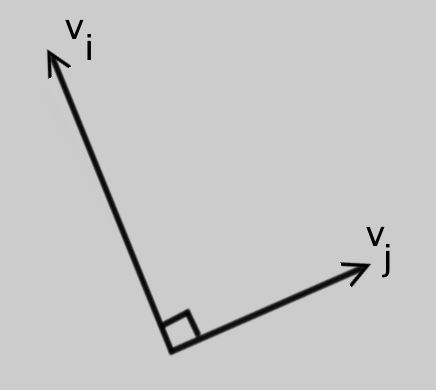
\includegraphics[scale=.4]{\orthonormPath/rightangles.jpg}
\end{center}
However, the basis is {\it not} orthonormal so we know nothing about the
lengths of the basis vectors (save that they cannot vanish). 

To complete the hint, lets use the dot product to compute a formula for $c^1$ in terms of the basis vectors and $v$. Consider
$$
v_1\dotprod v = c^1 v_1\dotprod v_1 + c^2 v_1\dotprod v^2 +\cdots + c^n v_1\dotprod v_n=c^1 v_1\dotprod v_1\, .
$$
Solving for $c^1$ (remembering that $v_1\dotprod v_1\neq 0$) gives
$$
c^1 = \frac{v_1\dotprod v\ }{v_1\dotprod v_1}\, .
$$
This should get you started on this problem.

} % Closing bracket for font

%\newpage


%\subsection*{\gaussElimTitle: Augmented Matrix Notation}
\subsection*{Augmented Matrix Notation}

%%%Insert this to get the typewriter font so it looks like a real movie script
{\ttfamily
\fontdimen2\font=0.4em
\fontdimen3\font=0.2em
\fontdimen4\font=0.1em
\fontdimen7\font=0.1em
\hyphenchar\font=`\-


%%%%put a hypertarget around the opening bit of text
\hypertarget{script_gaussian_elimination_more}{Why is the augmented  matrix} 
$$ \left( \begin{array}{cc | c}
1 & 1 & 27 \\
2 & -1 & 0  
\end{array} \right)\, ,
$$
equivalent to the system of equations
\begin{eqnarray*}
 x+y &=& 27\\
 2x - y &=& 0\, ?
\end{eqnarray*}
Well the augmented matrix is just a new notation for the matrix equation
\begin{equation*}
    \begin{pmatrix}
      1             &1  \\
      2             &-1
    \end{pmatrix}
  \colvec{x \\ y}
  =
  \colvec{27 \\ 0}
\end{equation*}
and if you review your matrix multiplication remember that 
\begin{equation*}
    \begin{pmatrix}
      1             &1  \\
      2             &-1
    \end{pmatrix}
  \colvec{x \\ y}
  =
  \colvec{x+ y \\ 2x - y}
\end{equation*}
This means that

\begin{equation*}
  \colvec{x+ y \\ 2x - y}
  =
  \colvec{27 \\ 0}\, ,
\end{equation*}
which is our original equation.

%%%%don't forget to close the bracket so the stuff after your file doesn't look like a movie!
}



\subsection*{Equivalence of Augmented Matrices}

%%%Insert this to get the typewriter font so it looks like a real movie script
{\ttfamily
\fontdimen2\font=0.4em
\fontdimen3\font=0.2em
\fontdimen4\font=0.1em
\fontdimen7\font=0.1em
\hyphenchar\font=`\-


%%%%put a hypertarget around the opening bit of text
\hypertarget{script_gaussian_elimination_background}{Lets think about what it means for the two augmented matrices} 


$$ \left( \begin{array}{cc | c}
1 & 1 & 27 \\
2 & -1 & 0  
\end{array} \right)
\mbox{ and } \left( \begin{array}{cc | c}
1 & 0 & 9 \\
0 & 1 & 18  
\end{array} \right)
$$
to be equivalent:
They are certainly not equal, because they don't match in each component, but since these augmented matrices represent a system, we might want to introduce a new kind of equivalence relation.

Well we could look at the system of linear equations this represents 

\begin{eqnarray*}
 x+y &=& 27\\
 2x - y &=& 0\, 
\end{eqnarray*}
and notice that the solution is $x=9$ and $y=18$. The other augmented matrix represents the system 
\begin{eqnarray*}
 x\ +0 \cdot y &=& 9\\
 0 \cdot x \ +\   \phantom{0 \cdot} y  &=& 18\, 
\end{eqnarray*}
This clearly has the same solution. The first and second system are related in the sense that their solutions are the same. Notice that it is really nice to have the augmented matrix in the second form, because the matrix multiplication can be done in your head.


%%%%don't forget to close the bracket so the stuff after your file doesn't look like a movie!
}

%\newpage


\subsection*{Hint for Review  Question~\ref{orthogprob}}

%%%Insert this to get the typewriter font so it looks like a real movie script
{\ttfamily
\fontdimen2\font=0.4em
\fontdimen3\font=0.2em
\fontdimen4\font=0.1em
\fontdimen7\font=0.1em
\hyphenchar\font=`\-


You are asked to consider an orthogonal basis $\{v_1,v_2,\ldots v_n\}$.
Because this is a basis any $v\in V$ can be uniquely expressed as
$$
v=c^1 v_1 + c^2 v_2 +\cdots +v^n c_n\, ,
$$
and the number $n=\dim V$. Since this is an orthogonal basis
$$
v_i\dotprod v_j =0 \, ,\qquad i\neq j\, .
$$
So different vectors in the basis are orthogonal:
\begin{center}
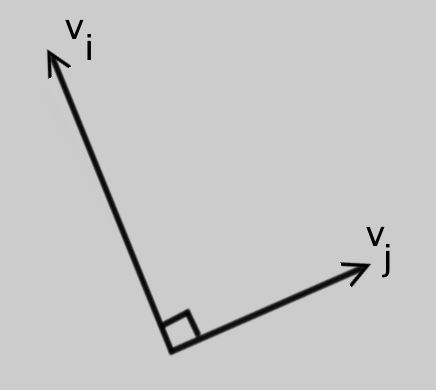
\includegraphics[scale=.4]{\orthonormPath/rightangles.jpg}
\end{center}
However, the basis is {\it not} orthonormal so we know nothing about the
lengths of the basis vectors (save that they cannot vanish). 

To complete the hint, lets use the dot product to compute a formula for $c^1$ in terms of the basis vectors and $v$. Consider
$$
v_1\dotprod v = c^1 v_1\dotprod v_1 + c^2 v_1\dotprod v^2 +\cdots + c^n v_1\dotprod v_n=c^1 v_1\dotprod v_1\, .
$$
Solving for $c^1$ (remembering that $v_1\dotprod v_1\neq 0$) gives
$$
c^1 = \frac{v_1\dotprod v\ }{v_1\dotprod v_1}\, .
$$
This should get you started on this problem.

} % Closing bracket for font

%\newpage



\subsection{\gaussElimTitle: $3 \times 3$ Example}

{\ttfamily
\fontdimen2\font=0.4em
\fontdimen3\font=0.2em
\fontdimen4\font=0.1em
\fontdimen7\font=0.1em
\hyphenchar\font=`\-

\hypertarget{scripts_gaussian_elimination_3_3_example}{We'll start with the matrix} from the \hyperlink{scripts_what_is_linear_algebra_3_3_matrix}{What is Linear Algebra: $3 \times 3$ Matrix Example} which was
\[
\begin{pmatrix}
5 & 10 & 25 & \vline & 65\\
1 & 1 & 1 & \vline & 7 \\
0 & -1 & 2 & \vline & 0
\end{pmatrix},
\]
and recall the solution to the problem was $n = 4$, $d = 2$, and $q = 1$. So as a matrix equation we have
\[
\begin{pmatrix}1 & 0 & 0 \\ 0 & 1 & 0 \\ 0 & 0 & 1\end{pmatrix} \begin{pmatrix}n \\ d \\ q\end{pmatrix} = \begin{pmatrix}4 \\ 2 \\ 1 \end{pmatrix}
\]
or as an augmented matrix
\[
\begin{pmatrix}
1 & & & \vline & 4 \\
& 1 & & \vline & 2 \\
& & 1 & \vline & 1
\end{pmatrix}
\]

Note that often in diagonal matrices people will either omit the zeros or write in a single large zero. Now
the first matrix is equivalent to the second matrix and is written as
\[
\begin{pmatrix}
5 & 10 & 25 & \vline & 65\\
1 & 1 & 1 & \vline & 7 \\
0 & -1 & 2 & \vline & 0
\end{pmatrix},
\sim
\begin{pmatrix}
1 & & & \vline & 4 \\
& 1 & & \vline & 2 \\
& & 1 & \vline & 1
\end{pmatrix}
\]
since they have the same solutions.


} % Closing brace for the font

\newpage



\subsection*{Worked Example}

%%%Insert this to get the typewriter font so it looks like a real movie script
{\ttfamily
\fontdimen2\font=0.4em
\fontdimen3\font=0.2em
\fontdimen4\font=0.1em
\fontdimen7\font=0.1em
\hyphenchar\font=`\-


\hypertarget{basis_and_dimension_example}{In this} 
video we will work through an example of how to extend a set of linearly independent vectors to a basis. For fun, we will take
the vector space 
$$
V=\{(x,y,z,w)|x,y,z,w\in {\mathbb Z}^5\}\, .
$$
This is like four dimensional space ${\mathbb R}^4$ except that the numbers can only be $\{0,1,2,3,4\}$. This is like bits, but now the rule is
$$
0=5\, .
$$
Thus, for example,  $\frac14=4$ because $4\time 4=16=1+3\times 5=1$. Don't get too caught up on this aspect, its a choice of base field designed
to make computations go quicker!

Now, here's the problem we will solve:

\begin{center}
{\bf Find a basis for $V$ that includes the vectors $\begin{pmatrix}1\\2\\3\\4\end{pmatrix}$ and $\begin{pmatrix}0\\3\\2\\1\end{pmatrix}$.}
\end{center}

The way to proceed is to add a known (and preferably simple) basis to the vectors given, thus we consider
\[
v_1=\begin{pmatrix}1\\2\\3\\4\end{pmatrix},\
v_2=\begin{pmatrix}0\\3\\2\\1\end{pmatrix},\
e_1=\begin{pmatrix}1\\0\\0\\0\end{pmatrix},\
e_2=\begin{pmatrix}0\\1\\0\\0\end{pmatrix},\
e_3=\begin{pmatrix}0\\0\\1\\0\end{pmatrix},\
e_4=\begin{pmatrix}0\\0\\0\\1\end{pmatrix}.
\]
The last four vectors are clearly a basis (make sure you understand this....) and are called the {\it canonical basis}\index{Canonical basis}.
We want to keep $v_1$ and $v_2$ but find a way to turf out two of the vectors in the canonical basis leaving us
a basis of four vectors. To do that, we have to study linear independence, or in other words a linear system problem
defined by
$$
0=\alpha_1 e_1 + \alpha_2 e_2 + \alpha_3 v_1 + \alpha_4 v_2 + \alpha_5 e_3 + \alpha_6 e_4 \, .
$$
We want to find solutions for the $\alpha's$ which allow us to determine two of the $e's$.
For that we use an augmented matrix
$$
\left(\begin{array}{cccccc|c}
1&0&1&0&0&0&0\\
2&3&0&1&0&0&0\\
3&2&0&0&1&0&0\\
4&1&0&0&0&1&0
\end{array}\right)\, .
$$
Next comes a bunch of row operations. Note that we have dropped the last column of zeros since it has no information--you can fill in the 
row operations used above the $\sim$'s as an exercise:
$$
\begin{pmatrix}
1&0&1&0&0&0\\
2&3&0&1&0&0\\
3&2&0&0&1&0\\
4&1&0&0&0&1
\end{pmatrix}\sim
\begin{pmatrix}
1&0&1&0&0&0\\
0&3&3&1&0&0\\
0&2&2&0&1&0\\
0&1&1&0&0&1
\end{pmatrix}
$$
$$
\sim
\begin{pmatrix}
1&0&1&0&0&0\\
0&1&1&2&0&0\\
0&2&2&0&1&0\\
0&1&1&0&0&1
\end{pmatrix}
\sim
\begin{pmatrix}
1&0&1&0&0&0\\
0&1&1&2&0&0\\
0&0&0&1&1&0\\
0&0&0&3&0&1
\end{pmatrix}
$$
$$
\sim
\begin{pmatrix}
1&0&1&0&0&0\\
0&1&1&0&3&0\\
0&0&0&1&1&0\\
0&0&0&0&2&1
\end{pmatrix}
\sim
\begin{pmatrix}
1&0&1&0&0&0\\
0&1&1&0&3&0\\
0&0&0&1&1&0\\
0&0&0&0&1&3
\end{pmatrix}
$$
$$
\sim
\begin{pmatrix}
\underline1&0&1&0&0&0\\
0&\underline1&1&0&0&1\\
0&0&0&\underline1&0&2\\
0&0&0&0&\underline1&3
\end{pmatrix}
$$
The pivots are underlined.
The columns corresponding to non-pivot variables are the ones that can be eliminated--their coefficients (the $\alpha$'s)
will be arbitrary, so set them all to zero save for the one next to the vector you are solving for which can be taken to be unity.
Thus that vector can certainly be expressed in terms of previous ones. Hence, altogether, our basis is
$$
\left\{
\begin{pmatrix}1\\2\\3\\4\end{pmatrix} \, , \ 
\begin{pmatrix}0\\3\\2\\1\end{pmatrix} ,\
\begin{pmatrix}0\\1\\0\\0\end{pmatrix} ,\
\begin{pmatrix}0\\0\\1\\0\end{pmatrix}
\right\}\, .
$$
Finally, as a check, note that $e_1=v_1+v_2$ which explains why we had to throw it away.



} % Closing bracket for font

%\newpage



\subsection*{Worked Examples of Gaussian Elimination}

{\ttfamily
\fontdimen2\font=0.4em
\fontdimen3\font=0.2em
\fontdimen4\font=0.1em
\fontdimen7\font=0.1em
\hyphenchar\font=`\-

\hypertarget{scripts_elementary_row_operations_worked_examples}{Let us consider that we are} given two systems of equations that give rise to the following two (augmented) matrices:
\begin{align*}
\begin{pmatrix}
2 & 5 & 2 & 0 & \vline & 2 \\
1 & 1 & 1 & 0 & \vline & 1 \\
1 & 4 & 1 & 0 & \vline & 1
\end{pmatrix}
\quad\quad
\begin{pmatrix}
5 & 2 & \vline & 9 \\
0 & 5 & \vline & 10 \\
0 & 3 & \vline & 6
\end{pmatrix}
\end{align*}
and we want to find the solution to those systems. We will do so by doing Gaussian elimination.

For the first matrix we have
\begin{align*}
\begin{pmatrix}
2 & 5 & 2 & 0 & \vline & 2 \\
1 & 1 & 1 & 0 & \vline & 1 \\
1 & 4 & 1 & 0 & \vline & 1
\end{pmatrix}
\overset{R_1 \leftrightarrow R_2}{\sim} &
\begin{pmatrix}
1 & 1 & 1 & 0 & \vline & 1 \\
2 & 5 & 2 & 0 & \vline & 2 \\
1 & 4 & 1 & 0 & \vline & 1
\end{pmatrix}
\\ \overset{R_2 - 2 R_1 ; R_3 - R_1}{\sim} &
\begin{pmatrix}
1 & 1 & 1 & 0 & \vline & 1 \\
0 & 3 & 0 & 0 & \vline & 0 \\
0 & 3 & 0 & 0 & \vline & 0
\end{pmatrix}
\\ \overset{\frac{1}{3}R_2}{\sim} &
\begin{pmatrix}
1 & 1 & 1 & 0 & \vline & 1 \\
0 & 1 & 0 & 0 & \vline & 0 \\
0 & 3 & 0 & 0 & \vline & 0
\end{pmatrix}
\\ \overset{R_1 - R_2 ; R_3 - 3 R_2}{\sim} &
\begin{pmatrix}
1 & 0 & 1 & 0 & \vline & 1 \\
0 & 1 & 0 & 0 & \vline & 0 \\
0 & 0 & 0 & 0 & \vline & 0
\end{pmatrix}
\end{align*}
\begin{enumerate}[1.]
\item We begin by interchanging the first two rows in order to get a 1 in the upper-left hand corner and avoiding dealing with fractions.

\item Next we subtract row 1 from row 3 and twice from row 2 to get zeros in the left-most column.

\item Then we scale row 2 to have a 1 in the eventual pivot.

\item Finally we subtract row 2 from row 1 and three times from row 2 to get it into Reduced Row  Echelon Form.
\end{enumerate}
Therefore we can write $x = 1 - \lambda$, $y = 0$, $z = \lambda$ and $w = \mu$, or in vector form
\[
\begin{pmatrix}x\\y\\z\\w\end{pmatrix} = \begin{pmatrix}1\\0\\0\\0\end{pmatrix} + \lambda \begin{pmatrix}-1\\0\\1\\0\end{pmatrix} + \mu \begin{pmatrix}0\\0\\0\\1\end{pmatrix}.
\]

Now for the second system we have
\begin{align*}
\begin{pmatrix}
5 & 2 & \vline & 9 \\
0 & 5 & \vline & 10 \\
0 & 3 & \vline & 6
\end{pmatrix}
\overset{\frac{1}{5}R_2}{\sim} &
\begin{pmatrix}
5 & 2 & \vline & 9 \\
0 & 1 & \vline & 2 \\
0 & 3 & \vline & 6
\end{pmatrix}
\\ \overset{R_3 - 3 R_2}{\sim} &
\begin{pmatrix}
5 & 2 & \vline & 9 \\
0 & 1 & \vline & 2 \\
0 & 0 & \vline & 0
\end{pmatrix}
\\ \overset{R_1 - 2 R_2}{\sim} &
\begin{pmatrix}
5 & 0 & \vline & 5 \\
0 & 1 & \vline & 2 \\
0 & 0 & \vline & 0
\end{pmatrix}
\\ \overset{\frac{1}{5}R_1}{\sim} &
\begin{pmatrix}
1 & 0 & \vline & 1 \\
0 & 1 & \vline & 2 \\
0 & 0 & \vline & 0
\end{pmatrix}
\end{align*}
We scale the second and third rows appropriately in order to avoid fractions, then subtract the corresponding rows as before. Finally scale the first row and hence we have $x = 1$ and $y = 2$ as a unique solution.

} % Closing brace for the font

%\newpage



\subsection{\elemRowOpsTitle: Explanation of Proof for Theorem~\ref{GJEunique}}

{\ttfamily
\fontdimen2\font=0.4em
\fontdimen3\font=0.2em
\fontdimen4\font=0.1em
\fontdimen7\font=0.1em
\hyphenchar\font=`\-

\hypertarget{scripts_elementary_row_operations_proof}{The first thing to realize is that} 
there are choices in the Gaussian elimination recipe, so maybe that could lead to two different
RREF's and in turn two different solution sets for the same linear system. But that would be weird,
in fact this Theorem says that this can never happen!

Because this proof comes at the end of the section it is often glossed over, but it is a very important result.
Here's a sketch of what happens in the video:
\begin{center}
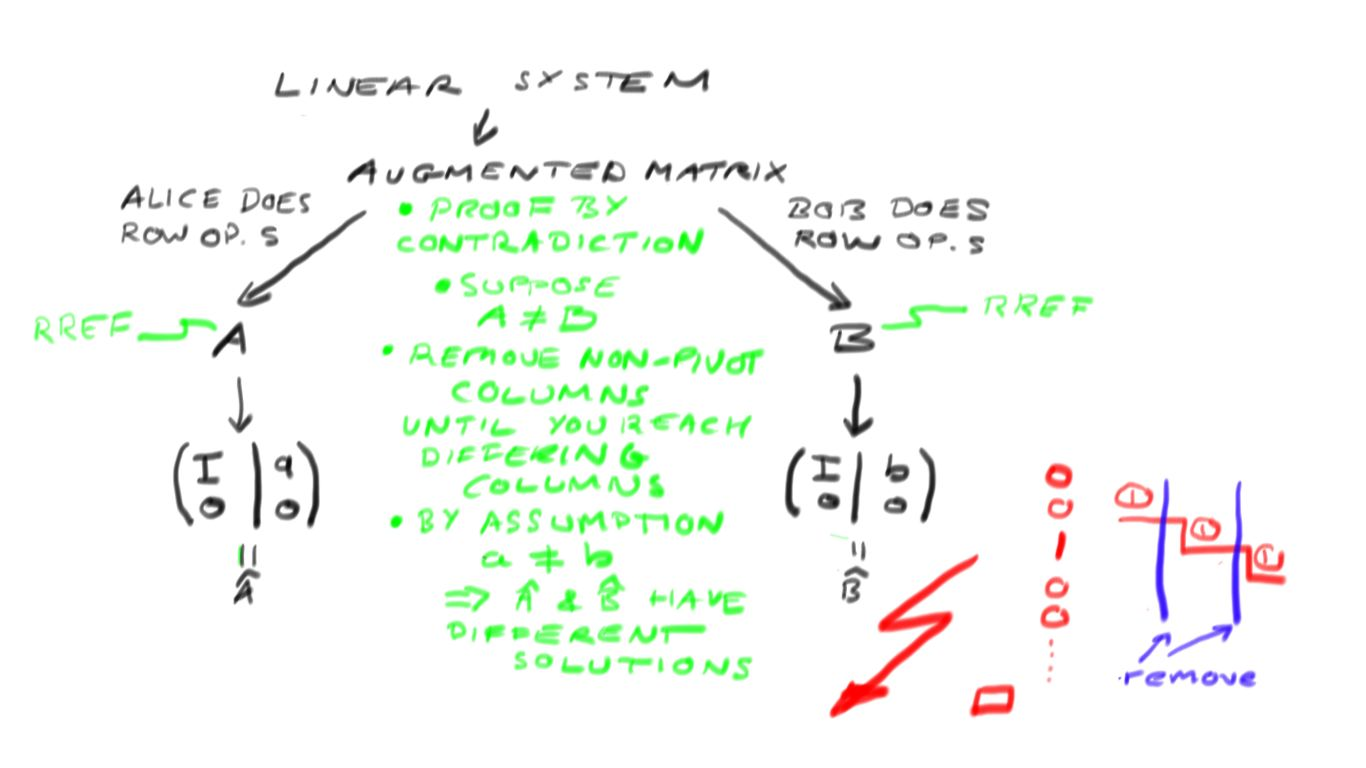
\includegraphics[scale=.3]{RREF_unique.jpg}
\end{center}

In words: we start with a linear system and convert it to an augmented matrix. Then, because we are studying a uniqueness
statement, we try a proof by contradiction. That is the  method where to show that a statement is true, you try to demonstrate that
the opposite of the statement leads to a contradiction. Here, the opposite statement to the theorem would be to find
two different RREFs for the same system.

Suppose, therefore, that Alice and Bob do find different RREF augmented matrices called $A$ and $B$. 
Then remove all the non-pivot columns  from $A$ and $B$  until you hit the first column that differs. Record that in the last column
and call the results $\widehat A$ and $\widehat B$. Removing columns
does change the solution sets, but it does not ruin row equivalence, so  $\widehat A$ and $\widehat B$ have the same solution sets.

Now, because we left only the pivot columns (plus the first column that differs) we have
$$\hat{A}=\begin{amatrix}{1}
I_N & a\\
0 & 0
\end{amatrix} \mbox{ and } \hat{B}=\begin{amatrix}{1}
I_N & b\\
0 & 0
\end{amatrix}\, ,$$ where $I_N$ is an identity matrix and $a$ and $b$ are column vectors.
Importantly, by assumption,
$$
a\neq b\, .
$$
So if we try to wrote down the solution sets for $\widehat A$ and $\widehat B$ they would be different.
But at all stages, we only performed operations that kept Alice's solution set the same as Bob's.
This is a contradiction so the proof is complete.
} % Closing brace for the font

\newpage



\subsection*{Hint for Review  Question~\ref{orthogprob}}

%%%Insert this to get the typewriter font so it looks like a real movie script
{\ttfamily
\fontdimen2\font=0.4em
\fontdimen3\font=0.2em
\fontdimen4\font=0.1em
\fontdimen7\font=0.1em
\hyphenchar\font=`\-


You are asked to consider an orthogonal basis $\{v_1,v_2,\ldots v_n\}$.
Because this is a basis any $v\in V$ can be uniquely expressed as
$$
v=c^1 v_1 + c^2 v_2 +\cdots +v^n c_n\, ,
$$
and the number $n=\dim V$. Since this is an orthogonal basis
$$
v_i\dotprod v_j =0 \, ,\qquad i\neq j\, .
$$
So different vectors in the basis are orthogonal:
\begin{center}
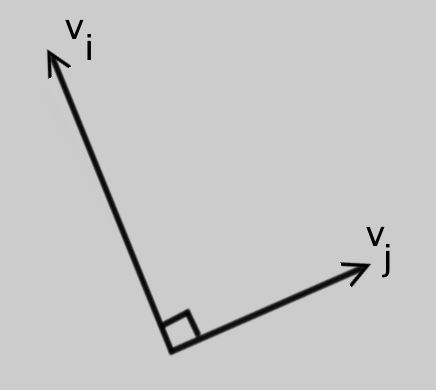
\includegraphics[scale=.4]{\orthonormPath/rightangles.jpg}
\end{center}
However, the basis is {\it not} orthonormal so we know nothing about the
lengths of the basis vectors (save that they cannot vanish). 

To complete the hint, lets use the dot product to compute a formula for $c^1$ in terms of the basis vectors and $v$. Consider
$$
v_1\dotprod v = c^1 v_1\dotprod v_1 + c^2 v_1\dotprod v^2 +\cdots + c^n v_1\dotprod v_n=c^1 v_1\dotprod v_1\, .
$$
Solving for $c^1$ (remembering that $v_1\dotprod v_1\neq 0$) gives
$$
c^1 = \frac{v_1\dotprod v\ }{v_1\dotprod v_1}\, .
$$
This should get you started on this problem.

} % Closing bracket for font

%\newpage



\subsection*{Planes}

%%%Insert this to get the typewriter font so it looks like a real movie script
{\ttfamily
\fontdimen2\font=0.4em
\fontdimen3\font=0.2em
\fontdimen4\font=0.1em
\fontdimen7\font=0.1em
\hyphenchar\font=`\-


%%%%put a hypertarget around the opening bit of text
\hypertarget{solution_sets_for_systems_of_linear_equations_planes}{Here we want} to describe the mathematics of planes in space.
The video is summarised by the following picture:
\begin{center}
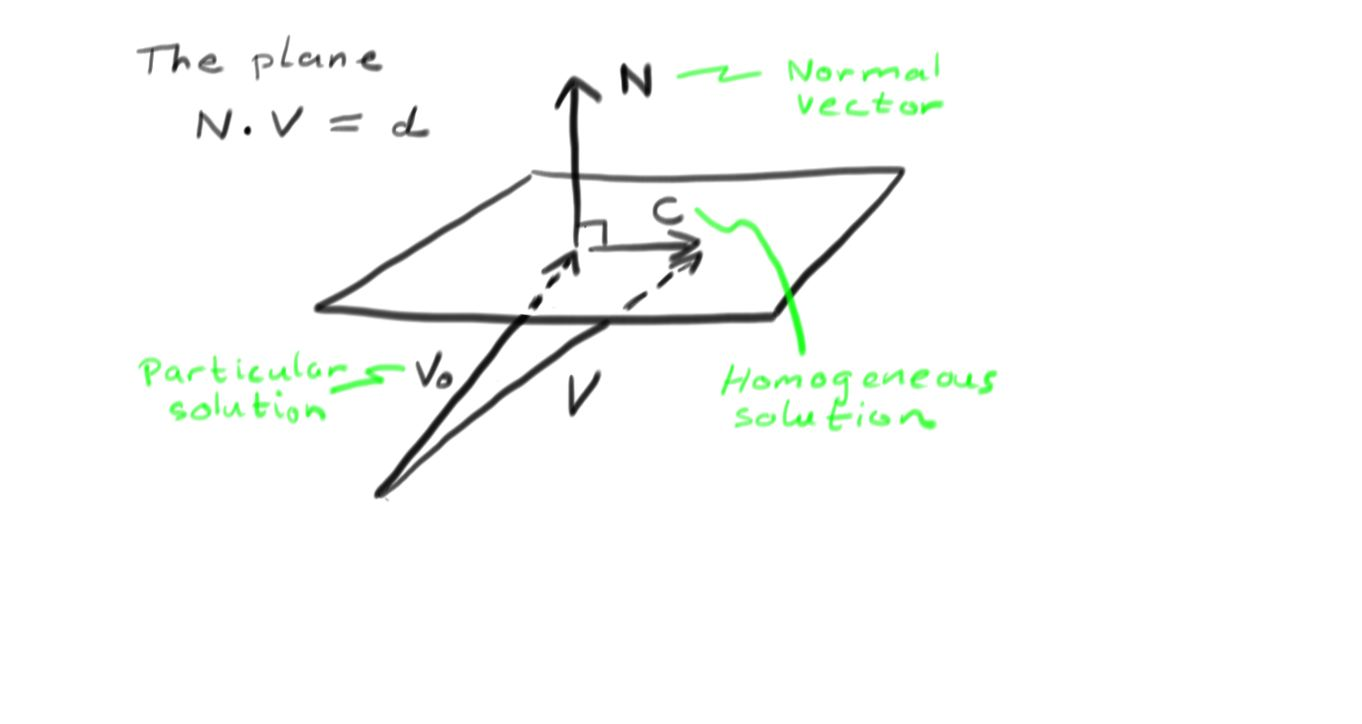
\includegraphics[scale=.2]{plane1eq.jpg}
\end{center}
A plane is often called ${\mathbb R}^2$ because it is spanned by  two coordinates, and space is called ${\mathbb R}^3$ and has three coordinates, 
usually called $(x,y,z)$. The equation for a plane is
$$
ax+by+cz=d\, .
$$
Lets simplify this by calling $V=(x,y,z)$ the vector of unknowns and $N=(a,b,c)$. Using the dot product in ${\mathbb R}^3$
we have
$$
N\dotprod V = d\, .
$$
Remember that when vectors are perpendicular their dot products vanish. {\it I.e.} $U\dotprod V = 0 \Leftrightarrow U \perp V$.
This means that if a vector $V_0$ solves our equation $N\dotprod V =d$, then so too does $V_0+C$ whenever $C$ is perpendicular to $N$.
This is because
$$N\dotprod (V_0+C) = N\dotprod V_0 + N\dotprod C = d + 0 = d\, .$$
But $C$ is ANY vector perpendicular to $N$, so all the possibilities for $C$ span a plane whose normal vector is $N$. Hence we have shown that 
solutions to the equation $ax+by+cz=0$ are a plane with normal vector $N=(a,b,c)$.



%%%%don't forget to close the bracket so the stuff after your file doesn't look like a movie!
}

%\newpage



\subsection{\whatIsTitle: Overview}

%%%Insert this to get the typewriter font so it looks like a real movie script
{\ttfamily
\fontdimen2\font=0.4em
\fontdimen3\font=0.2em
\fontdimen4\font=0.1em
\fontdimen7\font=0.1em
\hyphenchar\font=`\-


%%%%put a hypertarget around the opening bit of text
\hypertarget{video_what_is_overview}{In this course, we start with linear systems} 
\begin{equation}\label{linsys}
\left\{
\begin{array}{ccc}
f_1(x_1,\ldots,x_m)& = &a_1\\[1mm]
\vdots&&\vdots\\[1mm]
f_n(x_1,\ldots,x_m) &=& a_n\, ,
\end{array}
\right.
\end{equation}
and discuss how to solve them.

We end with the problem of finding a least squares fit---find the line that best fits a given data set:
\begin{center}
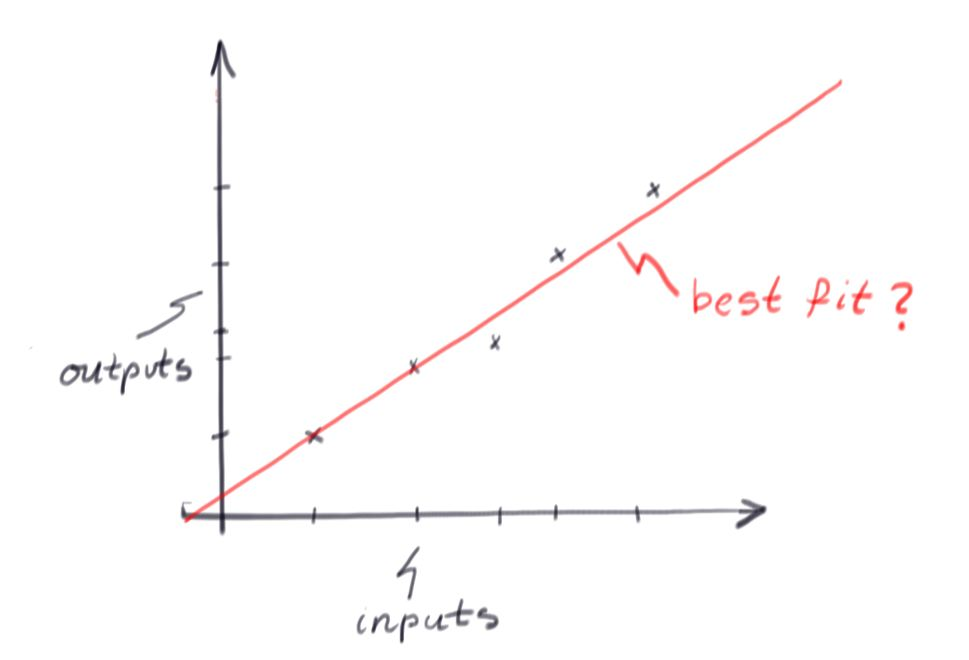
\includegraphics[scale=.2]{best_fit.jpg}
\end{center}

In equation~\eqref{linsys} we have $n$ {\it linear} functions called $f_1,\ldots, f_n$, $m$ un\-knowns $x_1,\ldots, x_m$
and $n$ given constants $a_1,\ldots,a_n$. We need to say what it means for a function to be linear.
A linear function has the {\it additive property}
$$
f(a+b)=f(a)+f(b)\, .
$$
The solution to this is
$$
f(x)=\lambda x\, ,
$$
for some constant $\lambda$. The plot of this is just a straight line through the origin with 
slope~$\lambda$
\begin{center}
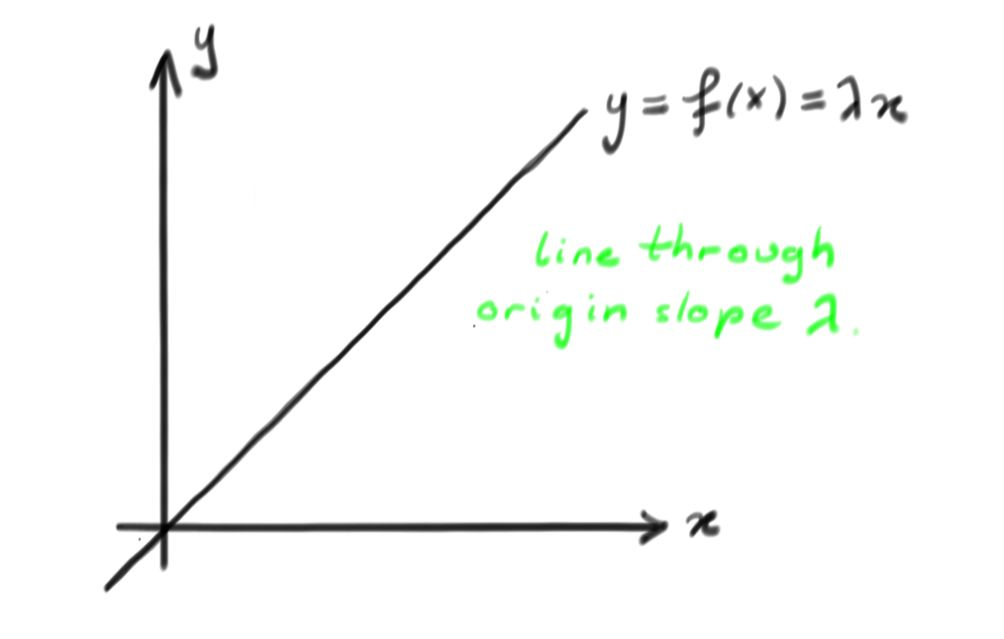
\includegraphics[scale=.2]{line_through_origin.jpg}
\end{center}

We should also check that our solution obeys the linearity property. The logic is to start with the left hand side $f(a+b)$
and try to turn it into the right hand side $f(a)+f(b)$ using correct manipulations:
$$
f(a+b)=\lambda(a+b) =\lambda a + \lambda b = f(a) + f(b)\, .
$$
The first step here just plugs $a+b$ into $f(x)$, the second is the distributive property, and in the third we recognize that $\lambda a = f(a)$ and $\lambda b = f(b)$.
This proves our claim.

For functions of many variables, linearity must hold for every slot. For a linear function of two variables $f(x,y)$ this means
$$
f(a+b,c+d)=f(a,c)+f(b,d)\, .
$$

We finish with a question. The plot of $f(x)=\lambda x + \beta$ is a straight line, but does it obey the linearity property?

%%%%don't forget to close the bracket so the stuff after your file doesn't look like a movie!
}

\newpage



\subsection*{Worked Example}

%%%Insert this to get the typewriter font so it looks like a real movie script
{\ttfamily
\fontdimen2\font=0.4em
\fontdimen3\font=0.2em
\fontdimen4\font=0.1em
\fontdimen7\font=0.1em
\hyphenchar\font=`\-


\hypertarget{basis_and_dimension_example}{In this} 
video we will work through an example of how to extend a set of linearly independent vectors to a basis. For fun, we will take
the vector space 
$$
V=\{(x,y,z,w)|x,y,z,w\in {\mathbb Z}^5\}\, .
$$
This is like four dimensional space ${\mathbb R}^4$ except that the numbers can only be $\{0,1,2,3,4\}$. This is like bits, but now the rule is
$$
0=5\, .
$$
Thus, for example,  $\frac14=4$ because $4\time 4=16=1+3\times 5=1$. Don't get too caught up on this aspect, its a choice of base field designed
to make computations go quicker!

Now, here's the problem we will solve:

\begin{center}
{\bf Find a basis for $V$ that includes the vectors $\begin{pmatrix}1\\2\\3\\4\end{pmatrix}$ and $\begin{pmatrix}0\\3\\2\\1\end{pmatrix}$.}
\end{center}

The way to proceed is to add a known (and preferably simple) basis to the vectors given, thus we consider
\[
v_1=\begin{pmatrix}1\\2\\3\\4\end{pmatrix},\
v_2=\begin{pmatrix}0\\3\\2\\1\end{pmatrix},\
e_1=\begin{pmatrix}1\\0\\0\\0\end{pmatrix},\
e_2=\begin{pmatrix}0\\1\\0\\0\end{pmatrix},\
e_3=\begin{pmatrix}0\\0\\1\\0\end{pmatrix},\
e_4=\begin{pmatrix}0\\0\\0\\1\end{pmatrix}.
\]
The last four vectors are clearly a basis (make sure you understand this....) and are called the {\it canonical basis}\index{Canonical basis}.
We want to keep $v_1$ and $v_2$ but find a way to turf out two of the vectors in the canonical basis leaving us
a basis of four vectors. To do that, we have to study linear independence, or in other words a linear system problem
defined by
$$
0=\alpha_1 e_1 + \alpha_2 e_2 + \alpha_3 v_1 + \alpha_4 v_2 + \alpha_5 e_3 + \alpha_6 e_4 \, .
$$
We want to find solutions for the $\alpha's$ which allow us to determine two of the $e's$.
For that we use an augmented matrix
$$
\left(\begin{array}{cccccc|c}
1&0&1&0&0&0&0\\
2&3&0&1&0&0&0\\
3&2&0&0&1&0&0\\
4&1&0&0&0&1&0
\end{array}\right)\, .
$$
Next comes a bunch of row operations. Note that we have dropped the last column of zeros since it has no information--you can fill in the 
row operations used above the $\sim$'s as an exercise:
$$
\begin{pmatrix}
1&0&1&0&0&0\\
2&3&0&1&0&0\\
3&2&0&0&1&0\\
4&1&0&0&0&1
\end{pmatrix}\sim
\begin{pmatrix}
1&0&1&0&0&0\\
0&3&3&1&0&0\\
0&2&2&0&1&0\\
0&1&1&0&0&1
\end{pmatrix}
$$
$$
\sim
\begin{pmatrix}
1&0&1&0&0&0\\
0&1&1&2&0&0\\
0&2&2&0&1&0\\
0&1&1&0&0&1
\end{pmatrix}
\sim
\begin{pmatrix}
1&0&1&0&0&0\\
0&1&1&2&0&0\\
0&0&0&1&1&0\\
0&0&0&3&0&1
\end{pmatrix}
$$
$$
\sim
\begin{pmatrix}
1&0&1&0&0&0\\
0&1&1&0&3&0\\
0&0&0&1&1&0\\
0&0&0&0&2&1
\end{pmatrix}
\sim
\begin{pmatrix}
1&0&1&0&0&0\\
0&1&1&0&3&0\\
0&0&0&1&1&0\\
0&0&0&0&1&3
\end{pmatrix}
$$
$$
\sim
\begin{pmatrix}
\underline1&0&1&0&0&0\\
0&\underline1&1&0&0&1\\
0&0&0&\underline1&0&2\\
0&0&0&0&\underline1&3
\end{pmatrix}
$$
The pivots are underlined.
The columns corresponding to non-pivot variables are the ones that can be eliminated--their coefficients (the $\alpha$'s)
will be arbitrary, so set them all to zero save for the one next to the vector you are solving for which can be taken to be unity.
Thus that vector can certainly be expressed in terms of previous ones. Hence, altogether, our basis is
$$
\left\{
\begin{pmatrix}1\\2\\3\\4\end{pmatrix} \, , \ 
\begin{pmatrix}0\\3\\2\\1\end{pmatrix} ,\
\begin{pmatrix}0\\1\\0\\0\end{pmatrix} ,\
\begin{pmatrix}0\\0\\1\\0\end{pmatrix}
\right\}\, .
$$
Finally, as a check, note that $e_1=v_1+v_2$ which explains why we had to throw it away.



} % Closing bracket for font

%\newpage



\subsection*{Hint for Review  Question~\ref{orthogprob}}

%%%Insert this to get the typewriter font so it looks like a real movie script
{\ttfamily
\fontdimen2\font=0.4em
\fontdimen3\font=0.2em
\fontdimen4\font=0.1em
\fontdimen7\font=0.1em
\hyphenchar\font=`\-


You are asked to consider an orthogonal basis $\{v_1,v_2,\ldots v_n\}$.
Because this is a basis any $v\in V$ can be uniquely expressed as
$$
v=c^1 v_1 + c^2 v_2 +\cdots +v^n c_n\, ,
$$
and the number $n=\dim V$. Since this is an orthogonal basis
$$
v_i\dotprod v_j =0 \, ,\qquad i\neq j\, .
$$
So different vectors in the basis are orthogonal:
\begin{center}
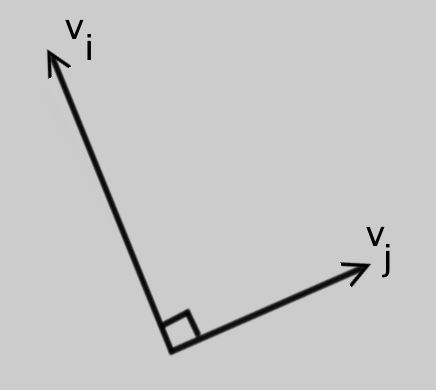
\includegraphics[scale=.4]{\orthonormPath/rightangles.jpg}
\end{center}
However, the basis is {\it not} orthonormal so we know nothing about the
lengths of the basis vectors (save that they cannot vanish). 

To complete the hint, lets use the dot product to compute a formula for $c^1$ in terms of the basis vectors and $v$. Consider
$$
v_1\dotprod v = c^1 v_1\dotprod v_1 + c^2 v_1\dotprod v^2 +\cdots + c^n v_1\dotprod v_n=c^1 v_1\dotprod v_1\, .
$$
Solving for $c^1$ (remembering that $v_1\dotprod v_1\neq 0$) gives
$$
c^1 = \frac{v_1\dotprod v\ }{v_1\dotprod v_1}\, .
$$
This should get you started on this problem.

} % Closing bracket for font

%\newpage


\newpage

\section*{Webwork Links}

\reading{1}{1}

\reading{1}{1}

\reading{2}{1}

\reading{2}{2}

\reading{3}{1}

\reading{4}{1}

\reading{4}{2}


\begin{center}\href{http://webwork.math.ucdavis.edu/webwork2/MAT22A-Waldron-Winter-2012/Homework0-Background/}{Background homework set}\end{center}

\begin{center}\href{http://webwork.math.ucdavis.edu/webwork2/MAT22A-Waldron-Winter-2012/Homework1-LinearSystems-waldron}{Linear Systems}\end{center}

\begin{center}\href{http://webwork.math.ucdavis.edu/webwork2/MAT22A-Waldron-Winter-2012/Homework2-SolnSets-Vectors-waldron/}{Solution Sets}\end{center}

\end{document}
